%
% First comes an example EPS file -- just ignore it and
% proceed on the \documentclass line
% your LaTeX will extract the file if required
\begin{filecontents*}{example.eps}
%!PS-Adobe-3.0 EPSF-3.0
%%BoundingBox: 19 19 221 221
%%CreationDate: Mon Sep 29 1997
%%Creator: programmed by hand (JK)
%%EndComments
gsave
newpath
  20 20 moveto
  20 220 lineto
  220 220 lineto
  220 20 lineto
closepath
2 setlinewidth
gsave
  .4 setgray fill
grestore
stroke
grestore
\end{filecontents*}
%
\RequirePackage{fix-cm}
%
% \documentclass{svjour3}                     % onecolumn (standard format)
%\documentclass[smallcondensed]{svjour3}     % onecolumn (ditto)
\documentclass[smallextended]{svjour3}       % onecolumn (second format)
%\documentclass[twocolumn]{svjour3}          % twocolumn
%
\smartqed  % flush right qed marks, e.g. at end of proof
%
\usepackage{graphicx}
\usepackage[most]{tcolorbox}
\usepackage{listings}
\usepackage{xcolor}
\usepackage{subcaption}
\usepackage{tabularx}
\usepackage{longtable}
\usepackage{booktabs}
\usepackage[colorinlistoftodos,prependcaption,textsize=tiny]{todonotes}
\usepackage{wrapfig}
\usepackage{framed}
\newcommand{\highlight}[1]{\begin{framed}%
  \noindent#1
\end{framed}}

\definecolor{backcolor}{rgb}{0.95,0.95,0.92}
\colorlet{punct}{red!60!black}
\definecolor{delim}{RGB}{20,105,176}
\colorlet{numb}{magenta!60!black}

\lstdefinestyle{mystyle}{
  language=Python,
  basicstyle=\ttfamily\footnotesize,
  keywordstyle=\color{delim},
  stringstyle=\color{punct},
  commentstyle=\color{numb},
  breakatwhitespace=true,
  breaklines=true,
  keepspaces=true,
  showspaces=false,
  showstringspaces=false,
  showtabs=false,
  tabsize=2,
  stepnumber=1,
  numbersep=3pt,
  captionpos=b,
  % numbers=left,
  % numberstyle=\tiny\color{gray},
  backgroundcolor=\color{backcolor},
  % aboveskip=0pt,
  % belowskip=0pt
}
\lstset{style=mystyle}

\lstset{emph={%
    assert%
    },emphstyle={\color{delim}}%
}%

%
% \usepackage{mathptmx}      % use Times fonts if available on your TeX system
%
% insert here the call for the packages your document requires
%\usepackage{latexsym}
% etc.
%
% please place your own definitions here and don't use \def but
% \newcommand{}{}
%
% Insert the name of "your journal" with
% \journalname{myjournal}
%
\begin{document}

\title{Exploring the Role of Feedback in Machine Learning Jupyter Notebooks}

%\titlerunning{Short form of title}        % if too long for running head

\author{Arumoy Shome\and
  Lu{\`\i}s Cruz\and
  Diomidis Spinellis\and
  Arie van Deursen
}

%\authorrunning{Short form of author list} % if too long for running head

\institute{A. Shome \at
  Delft University of Technology\\
  \email{a.shome@tudelft.nl}
  \and
  L. Cruz \at
  Delft University of Technology\\
  \email{l.cruz@tudelft.nl}
  \and
  D. Spinellis \at
  Delft University of Technology\\
  \email{d.spinellis@tudelft.nl}
  \and
  A. V. Deursen \at
  Delft University of Technology\\
  \email{arie.vandeursen@tudelft.nl}
}

\date{Received: date / Accepted: date}
% The correct dates will be entered by the editor


\maketitle

\begin{abstract}

  % TODO: update the abstract
  Developing and testing ML systems is a highly interactive process which demands a human-in-the-loop approach. In addition to writing tests for the code base, practitioners are required to analyse and interpret several visualisations using their domain expertise to validate if an ML system satisfies the required set of functional and non-functional properties. Visualisations are frequently used to qualitatively assess various parts of an ML pipeline. However, implicit knowledge gained from visualisations must be translated to explicit analytical tests that fail when there is change in any component of the ML pipeline. We conduct an empirical analysis of Jupyter notebooks to catalogue the state-of-the-art mappings between ML visualisations and assertions. We mine Github to collect 54K Jupyter Notebooks that contain assertions written in Python. We develop a novel methodology to identify 1764 notebooks which contain an assertion below a visualisation. We manually analyse the 1.7K notebooks and identify 269 visualisation-assertion pairs that are semantically related to one another. We further investigate the 269 visualisation-assertion pairs and identify three frequently occurring testing patterns. We perform an in-depth analysis of 34 visualisation-assertion pairs and find that the assertions often fail to capture all the information present in their visual counter-part. Empirical evidence obtained in this study indicates that current software testing methods fail to address the unique challenges of ML. And emphasises the need for automated tools that bridge the gap between visual assessments and analytical assertions.

\end{abstract}

\keywords{ML Testing \and SE4AI \and Visualisations \and Assertions \and Computational Notebooks}

\section{Introduction}
The machine learning development lifecycle (MLDL) encompasses a multifaceted series of entangled stages. Significant effort is invested in gathering and assembling the required data from diverse sources. The data then undergo cleaning and preprocessing to ensure high quality and usability, in the subsequent stages. MLDL is dominated by the model development phase which is highly experimental and iterative. This stage involves exploratory data analysis (EDA) to uncover underlying patterns, fitting the data to various models, and rigorously analysing the results. Often, this stage may lead to additional rounds of feature engineering, where new attributes are created based on insights gained from initial models to enhance model performance. Practitioners may also engage in comparing and contrasting different models to identify the most effective approach, followed by fine-tuning selected models to optimize performance. The final model is then deployed into production where it is continuously monitored, and periodically retrained to adapt to new data or changing conditions~\cite{haakman2021ai,amershi2019software,sculley2015hidden}.

The MLDL is fundamentally iterative, closely resembling Agile software engineering principles, which emphasize incorporating early feedback and working in small, manageable iterations~\cite{betz2018managing}. Similarly, CRISP-DM---the dominant process model in data mining---outlines a cyclical process that evolves from understanding the business objectives and data, data preparation, modelling, evaluation and finally deployment and monitoring~\cite{martinez-plumed2021crisp-dm}. Both systems advocate for a dynamic, iterative approach that enhances adaptability and effectiveness in dealing with complex, changing systems like those encountered in ML projects.

Computational notebooks---specifically Jupyter notebooks\footnote{https://jupyter.org/}---have been ubiquitously adopted by the ML community for developing ML enabled systems~\cite{pimentel2019large-scale,quaranta2021kgtorrent,psallidas2019data,perkel2018why}. Jupyter notebooks provide an interactive computing environment that allow users to break the development of complex workflows into smaller, more manageable code chunks. Each notebook is composed of a series of code cells, which can be executed independently in a read-eval-print loop (REPL) style of interactive software development. This REPL approach allows users to write a piece of code, run it, and immediately see the results thus facilitating an incremental and iterative style of software development. This modular structure of notebooks provides users the flexibility to experiment with different approaches and algorithms. Users can test hypotheses, debug issues, and make incremental changes with immediate feedback. The ability to visualize data and results inline and document the process in a narrative form further enhances their utility~\cite{kery2018story,head2019managing,rule2018exploration,chattopadhyay2020whats}.

% NOTE: consider starting with prints and last statements first (most obvious), then move to assertions; its fine if RQs follow different order
Jupyter notebooks are primarily used to explore different ideas or approaches, often neglecting software development best practices in favor of rapid experimentation~\cite{kery2018story,rule2018exploration,pimentel2019large-scale}. During this process, practitioners can use various feedback mechanisms like assertions, print statements, output of code cells and visualisations to determine the appropriate data preprocessing techniques, detect erroneous assumptions, create new features to boost model performance, and select specific hyperparameters~\cite{head2019managing,chattopadhyay2020whats}. Once the code is finalised, it is typically transferred into a script that is run in a production environment. Alternatively, the notebook may contain significant exploratory work such as developing a model or performing data exploration. To effectively communicate the information present in the notebooks with clients, collaborators or teammates, the practitioners add annotations and structure to the notebook using markdown cells~\cite{kery2018story,rule2018exploration}. In both scenarios, practitioners need to revisit the notebooks to obtain structured information such as up-to-date and accurate requirements, their rationale and design decisions, and tests---artifacts which are usually missing in the original notebooks~\cite{pimentel2019large-scale,psallidas2019data,grotov2022large-scale}. As data, personnel, and system environments inevitably change, undocumented decisions can lead to accumulation of technical debt. This not only prolongs time required for debugging and troubleshooting, but also incurs additional costs and resource expenditures~\cite{sculley2015hidden,amershi2019software,sambasivan2021everyone}.

% TODO: feedback from diomidis
% - "We identify a knowledge gap in the current approach used to obtain such structured information from experimental code within Jupyter notebooks." Rephrase to have the knowledge gap correspond to what the RQs answer.  Currently one may think that we aim to improve the approach, not its understanding.
We identify a knowledge gap in the current approach used to obtain such structured information from experimental code within Jupyter notebooks. To address this gap, this study conducts a series of empirical studies to understand the role of various feedback mechanisms used to develop ML pipelines within Jupyter notebooks. We focus on implicit form of feedback obtained from print statements and output generated by the last statement in code cells, as well as explicit form of feedback obtained from assertions. To the best of our knowledge, we are the first to investigate how such feedback mechanisms are used by ML practitioners when developing ML pipelines inside Jupyter notebooks. The research questions along with the contributions of this study are presented below.

\begin{description}
  \item[RQ1.] \textbf{What feedback mechanisms are employed in the development of ML Jupyter notebooks?}

    We mine 297.8 thousand Jupyter notebooks written in Python from Github and Kaggle. We analyse 2.3 million code cells obtained from the notebooks and create a public dataset of 27.1 thousand assertions, 498.3 thousand print statements and 373.6 thousand last statements. We perform a descriptive and lexical analysis of the dataset and report the key characteristics of feedback mechanisms used in ML Jupyter notebooks.

  % TODO: add citation for the dataset (make it public so that DOI is available)

  \item[RQ2.] \textbf{How is explicit feedback from assert statements used to validate ML code written in Jupyter notebooks?}

    To gain a deeper understanding of assert statements written in Jupter notebooks, we conduct individual case-studies with 82 assert statements. We analyse the assertion along with the surrounding code to understand its purpose. Additionally, we analyse the entire code cell, the previous and next cells along with the purpose of the notebook to bring in rich context.

  \item[RQ3.] \textbf{How is implicit feedback from print statements and last statements of code cells used when writing ML code in Jupyter notebooks?}

    Similarly, we conduct individual case-studies with 44 print statements and 27 last statements. During each case-study, we analyse the code statement along with the raw output to understand its purpose.
\end{description}

% TODO revisit this paragraph
% TODO what should be done to change the things we observe? to increase the use of explicit feedback? do we know if its important or not? maybe we need to explore that?
Our findings indicate that outputs from code cells are extensively utilised for making critical design and implementation decisions during the MLDL. While manual validation of these outputs is common, it is also prone to inconsistencies thus highlighting the need for automated validation mechanisms. Assertions are identified as a potential solution, capable of verifying data distributions and ensuring model performance metrics meet predefined thresholds, thereby reducing reliance on manual checks and enhancing the robustness of ML pipelines. However, the study also notes the limited use of assertions, with only 9.7\% of the 3 million notebooks analyzed incorporating them, suggesting a significant gap in current testing practices within the ML community. The findings underscore the necessity for developing ML-specific testing tools and integrating assertions more deeply into the ML development workflow to ensure consistent and reliable validation processes.

% TODO update replication package

% the replication package for this study is made public on figshare\footnote{the replication package can be found at this url: https://figshare.com/s/9347228011999cba29f5}.

\section{Background}\label{sec:background}

This section introduces relevant prior concepts for this study.

\subsection{REPLs, Interactive Computing and Project Jupyter}

A Read-Eval-Print Loop (REPL) is an interactive programming environment that takes single user inputs (Read), executes them (Eval), returns the result to the user (Print) and then waits for the next command (Loop). REPLs offer an immediate feedback loop for quickly testing and debugging code snippets. The Python standard distribution includes a Python REPL with a command line interface to execute Python code in real-time. IPython---a more advanced alternative to the Python REPL---extends the capabilities of the standard Python shell with additional features such as powerful introspection, additional shell syntax, tab completion, and command history. Jupyter notebooks (and its successor Jupyter lab) leverage the IPython kernel to execute Python code and extends its capabilities with a graphical user interface (GUI). Resembling the literate programming paradigm~\cite{knuth1984literate}, Jupyter notebooks offer a web-based interface where users can create and share documents that contain live code, equations, visualisations, and narrative text. This format supports a literate approach to programming, making it easier to share and understand complex analyses and workflows. Jupyter Notebooks in particular, have become a popular tool in the ML community since they facilitate open and reproducible science, education, and data analysis.

\subsection{Anatomy of Jupyter Notebooks}

\begin{figure}
  \centering
  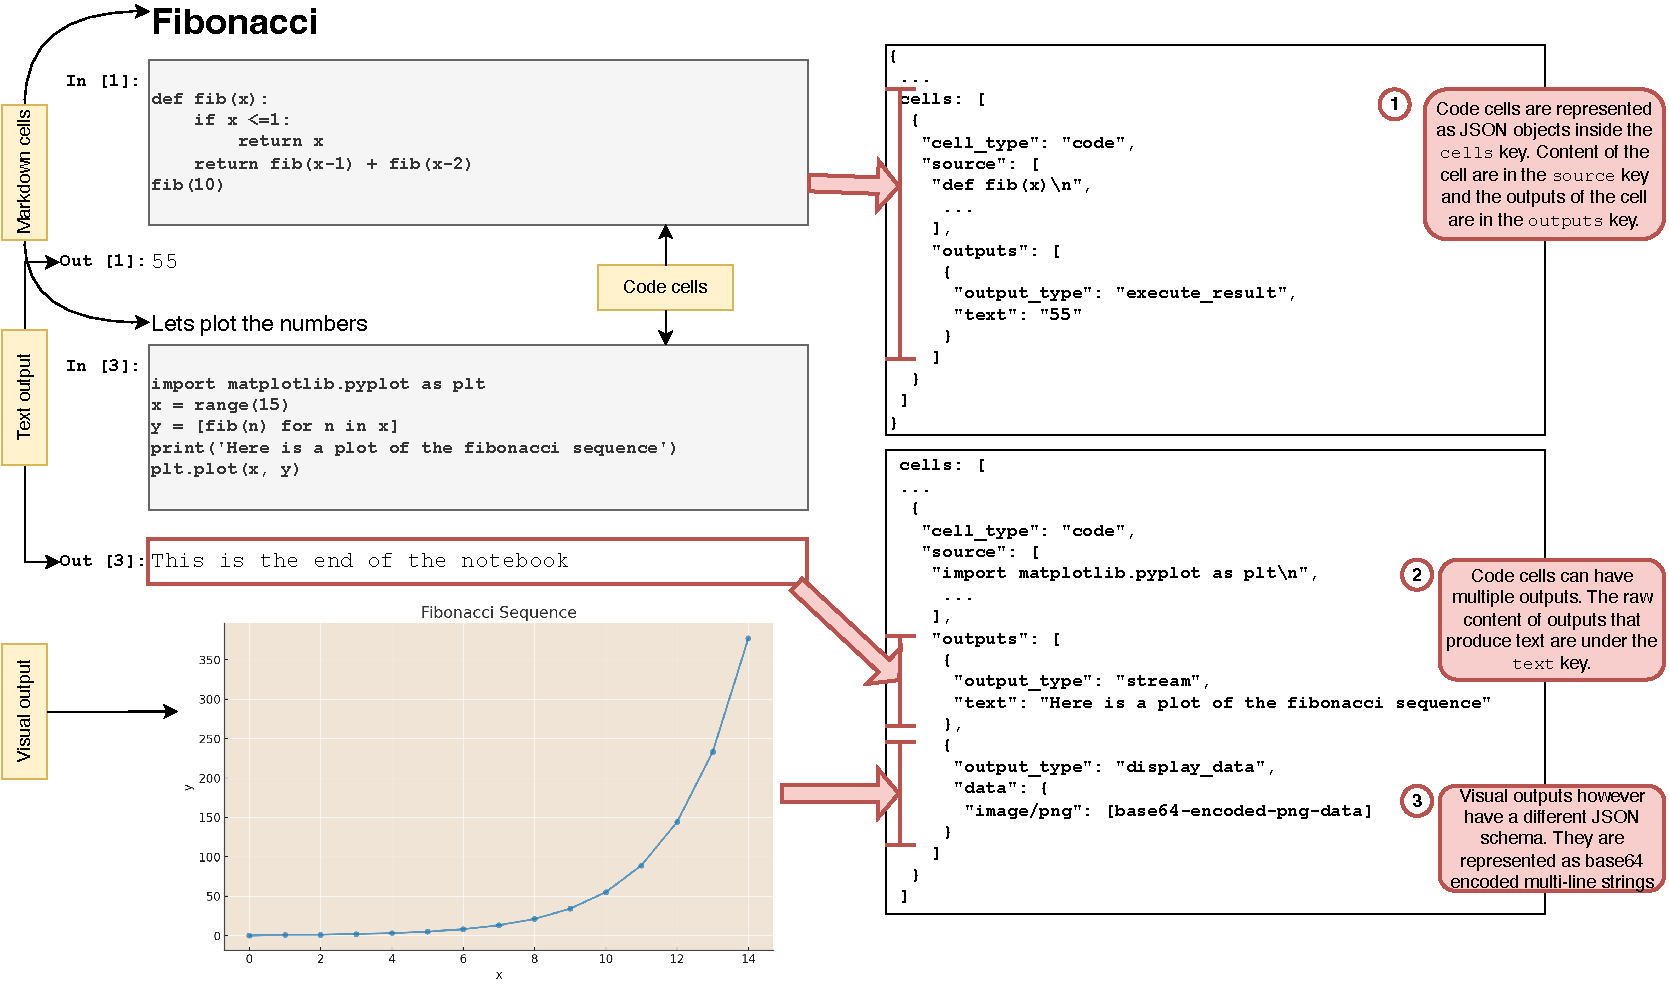
\includegraphics[width=\linewidth]{nb.pdf}
  \caption{Example Jupyter notebook with code and markdown cells, adapted ~\cite[Figure~1]{pimentel2019large-scale}.}
  \label{fig:nb}
\end{figure}

Figure~\ref{fig:nb} shows an example Jupyter notebook with markdown and code cells. The data comprised within Jupyter notebooks is stored using the JSON schema specified by \emph{nbformat}~\footnote{https://nbformat.readthedocs.io/en/latest/index.html}, and thus can be parsed programmatically. A notebook consists of \emph{cells} which can be of three types---``markdown'', ``code'' and ``raw''. All cells of a notebook are stored as a list under the top-level \lstinline[language={}]$cells$ key in the JSON representation. Within this list, each cell is represented as a JSON object. The contents of the cell are stored as a list of strings inside the \lstinline[language={}]$source$ key.

Only code cells in Jupyter notebooks can generate outputs. As shown in Figure~\ref{fig:nb}, outputs can come from three main sources in the source code---print statements, the last statement in the code cell, and statements that create a visualisation. The outputs produced by code cells are stored as JSON objects under the \lstinline[language={}]$outputs$ key in the corresponding JSON representation of the notebook. Text outputs (such as those produced by the last statement of a cell or print statements) are stored under the \lstinline[language={}]$text$ key. Visual outputs have a sightly different JSON schema and are stored under the \lstinline[language={}]$data$ key. The image itself is represented as a base64 encoded string which is stored inside the \lstinline[language={}]$data$ object, under the \lstinline[language={}]$image/png$ key.

\subsection{Python Abstract Syntax Tree}

The Python \lstinline{ast} module enables the parsing, manipulation, and analysis of Python source code by converting it into an abstract syntax tree (AST)~\cite{pythonast}. The \lstinline{ast} module can parse source code strings into AST objects, traverse and modify the tree, and compile it back into executable code, providing a powerful tool for dynamic code manipulation. In Python, \lstinline{assert} statements are represented in the AST by the \lstinline{Assert} class. The \lstinline{Assert} node includes the \lstinline{test} attribute---which contains the condition being asserted---and the \lstinline{msg} attribute---which holds an optional message displayed if the assertion fails. Print statements are treated as a call to the built-in \lstinline{print} function. Function calls are represented in the AST by the \lstinline{Call} class. The \lstinline{Call} node includes the \lstinline{func} attribute representing the \lstinline{print} function, and \lstinline{args} which lists the arguments passed.

\section{Methodology}

\subsection{Data Collection}\label{sec:data-collect}

\begin{figure}
  \centering
  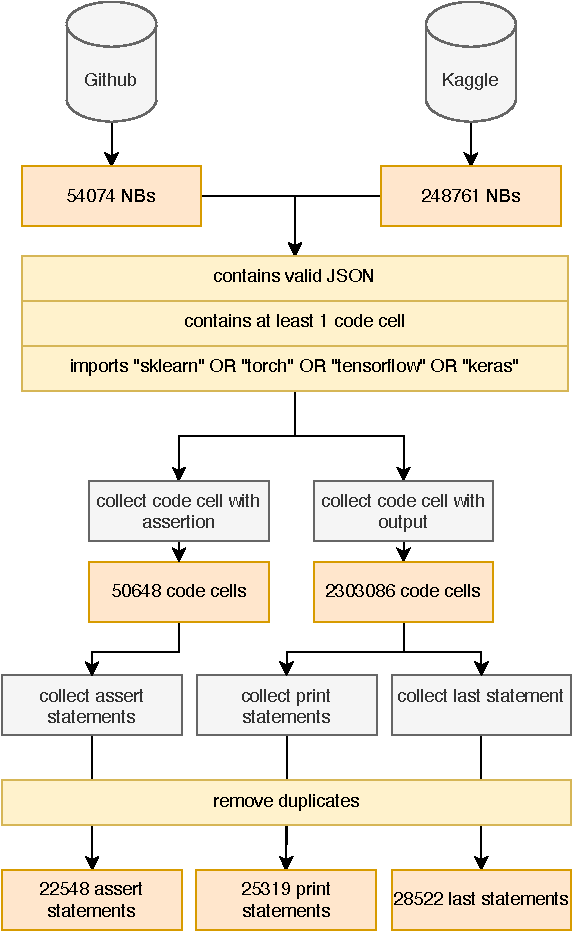
\includegraphics[width=0.75\linewidth]{data-collection.pdf}
  \caption{Overview of data collection methodology used in this study}
  \label{fig:data-collection}
\end{figure}

% TODO: I suspect this will raise eyebrows because the notebooks collected from Github were for the ICST paper, where we were also looking for the keyword "assert" (which does not apply to this paper)

Figure~\ref{fig:data-collection} illustrates the data collection process employed in this study to gather Jupyter notebooks written in Python from GitHub and Kaggle. We used Github's advanced search syntax~\footnote{https://docs.github.com/en/search-github/searching-on-github/searching-code}, with the following search query: \lstinline[language={}]$language:"Jupyter Notebook"$ to mine 49.9 thousand Jupyter notebooks from public repositories on Github~\footnote{Collected on June 22, 2023}. We used the pre-existing dataset KGTorrent~\cite{quaranta2021kgtorrent} for Kaggle since it does not support advanced code-based search like GitHub. To the best of our knowledge, KGTorrent is the largest dataset of Python Jupyter notebooks obtained from Kaggle, consisting of 247.9 thousand notebooks. Consequently, we started with 283GB of data comprising 297.8 thousand Python Jupyter notebooks.

Since the focus of this study is on the analysis of Python code, we only include notebooks that have a valid underlying JSON structure and contain at least one code cell. Finally, to focus on Python code written specifically for ML projects, we only include notebooks that import at least one of the following popular ML libraries which we identified from grey literature~\cite{datacampml,gfgml,jetbrainsml,kdnuggetml,courseraml}---Scikit Learn~\cite{virtanen2020scipy}, Pytorch~\cite{paszke2017automatic}, Tensorflow~\cite{abadi2015tensorflow} and Keras~\cite{chollet2015keras}. We use the Python \lstinline{ast} module to extract the assert, print and last statements from all code cells. Prior to conducting the analysis for RQ2 and RQ3, we remove duplicate data points resulting in a final data set of 27.1 thousand assertions, 498.3 thousand print statements and 373.6 thousand last statements.

\subsection{Case Studies}

We allocated a fixed time resource of 200 hours to conduct the case study analysis of all candidate assertions, print statements and last statements. To surface interesting candidates for the case studies, we apply text processing techniques as described below.

The assertions and cell outputs are first tokenised---special characters and alpha-numeric words shorter than two characters are removed. Two stop words namely ``assert'' and ``print'' are removed since they appear in all assertions and print statements respectively. The term frequency (TF) for all tokens is calculated and then normalised using their inter-document frequency (IDF) such that tokens that appear less frequently are assigned a higher value. We apply stratified random sampling to identify the candidates for the case study analysis. The sub-groups are created by adding TF-IDF of the tokens in each candidate to produce an aggregate value. The candidates are then divided into quartiles based on the aggregate value. A candidate is randomly drawn from each bin and analysed as an in-depth case study. The analysis is stopped when the time resource is exhausted. During each case study, we analyse the code of the candidate to understand its purpose. Additionally, we analyse the entire code cell, the previous cell, next cell and the notebook's purpose to bring in rich context.

\section{Results}

% TODO: feedback from Diomidis
% - Sections 4.1 and 4.2 are very interesting but overly detailed. I suggest to move most of the content to an appendix or an online appendix, and only present the uses in a table or a taxonomy tree.
% TODO: In addition, consider moving the more general observations into a discussion section.

\begin{figure}
  \centering
  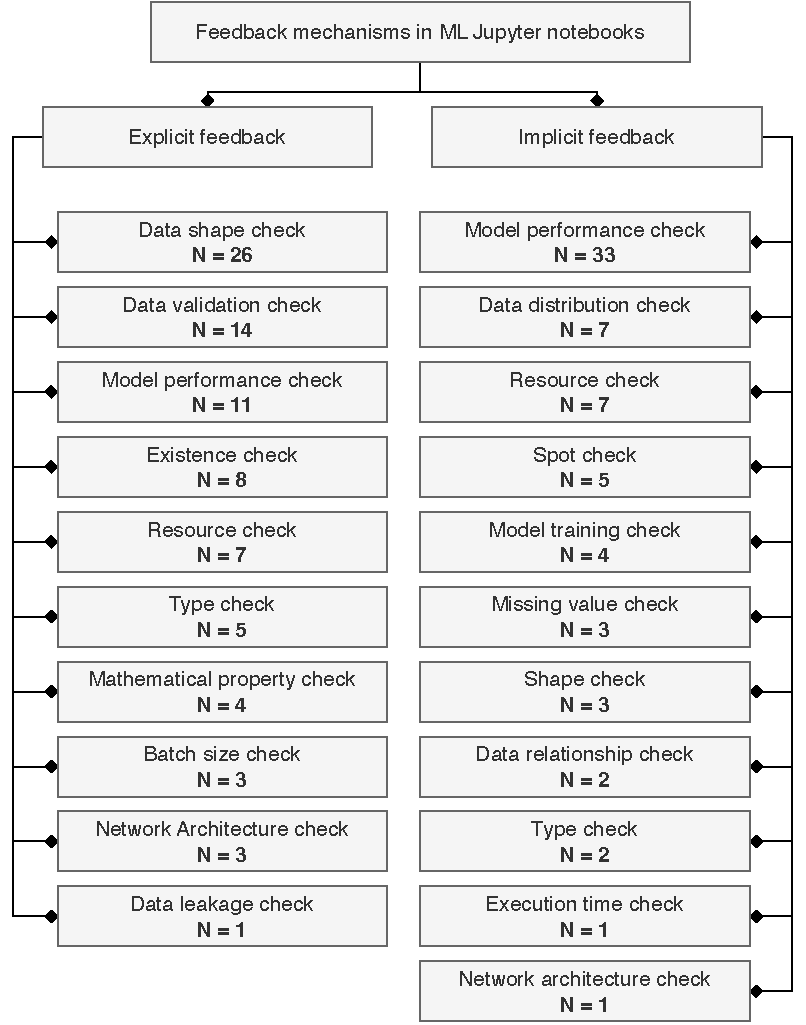
\includegraphics[width=0.75\textwidth]{taxonomy.pdf}
  \caption{Overview of various feedback mechanism groups identified in this study.}
  \label{fig:taxonomy}
\end{figure}

% TODO: add citation to online appendix
The results of the study are presented in this section. For the case-studies conducted for RQ2 and RQ3, we group the candidates based on their similarity to each other. Please note that this is done only to facilitate structuring the paper in a meaningful manner and for easy of reporting the results. Figure~\ref{fig:taxonomy} provides an overview of the various feedback mechanism groups identified in this study. Additional details are provided in Section~\ref{sec:result-explicit} and Section~\ref{sec:result-implicit}. Throughout the text, we reference the candidates (\textbf{(A)}ssertions, \textbf{(P)}rint statements and \textbf{(L)}ast cell statements) using their unique identifiers as examples. These can be viewed on our online appendix.

\subsection{(RQ1) What feedback mechanisms are employed in the development of ML Jupyter notebooks?}~\label{sec:result-analysis}

25 thousand (8.5\%) notebooks contained at least one assertion. From the 8.5\% notebooks, we collected 89.6 thousand assertions. 4.8 thousand assertions (5\%) used methods from external testing libraries. 85 thousand assertions (95\%) however were written using the \lstinline{assert} statement provided by the built-in Python standard library. We removed duplicate assertions for the remainder of the analysis, thus resulting in 27.1 thousand assertions.

\begin{figure}
  \centering
  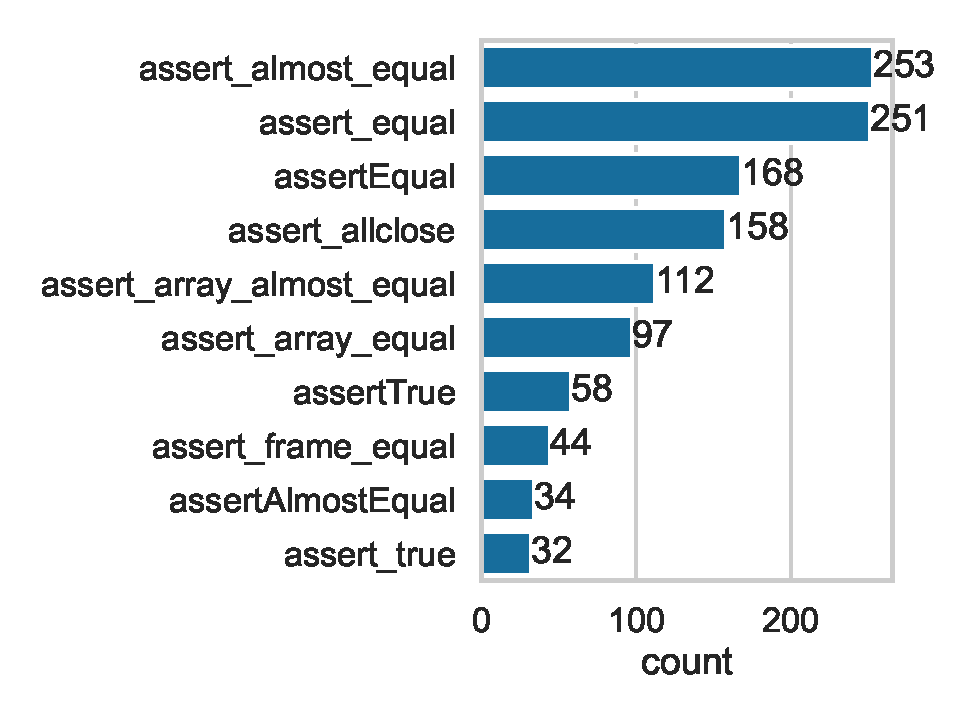
\includegraphics[width=0.5\textwidth]{other-test-methods.pdf}
  \caption{10 most common methods used in assertions written using external testing libraries.}
  \label{fig:other-test-methods}
\end{figure}

Figure~\ref{fig:other-test-methods} presents the 10 most common methods used in the 5\% assertions written using external testing libraries. We manually tracked the source of the methods to the numpy, pandas, torch and unittest libraries. The most frequently used methods include \lstinline{assert_almost_equal} and \lstinline{assert_equal}, each with over 250 instances. Methods such as \lstinline{assert_almost_equal}, \lstinline{assert_array_almost_equal} and \lstinline{AssertAlmostEqual} accommodate the stochastic nature of ML, where results can vary slightly due to inherent randomness in data processing and model training. We also find methods such as \lstinline{assert_array_equal} and \lstinline{assert_frame_equal} that are specifically tailored for comparing high-dimensional data structures such as numpy arrays and pandas data frames.

\begin{figure}
  \centering
  \begin{minipage}{0.49\textwidth}
    \centering
    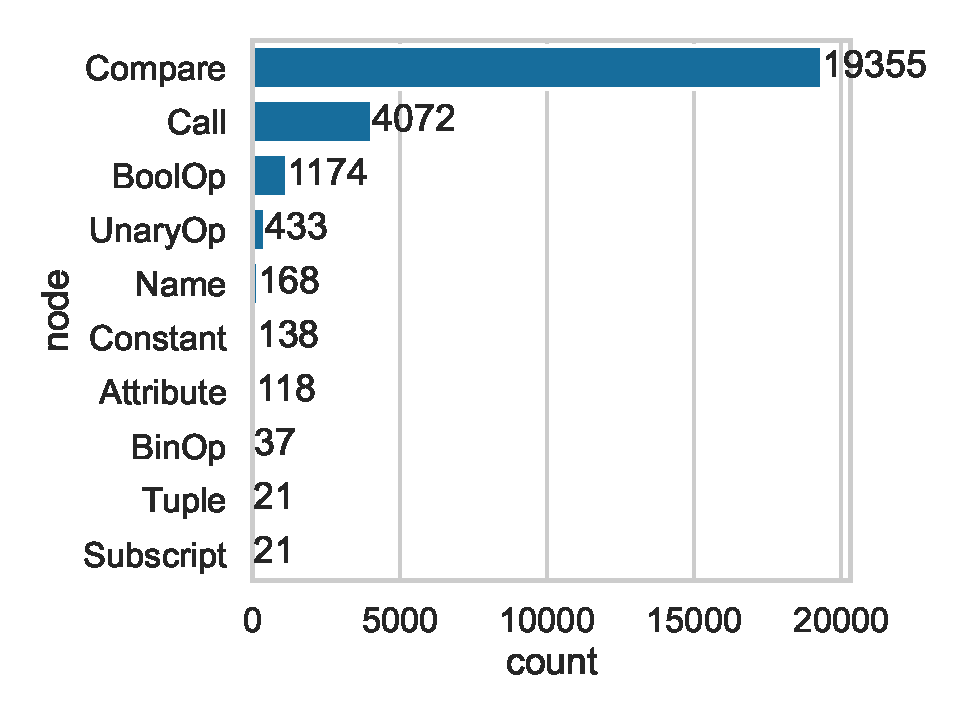
\includegraphics[width=\linewidth]{common-assert-test.pdf}
    \caption{10 most common tests used in \lstinline{assert} statements.}
    \label{fig:common-assert-test}
  \end{minipage}
  \hfill
  \begin{minipage}{0.49\textwidth}
    \centering
    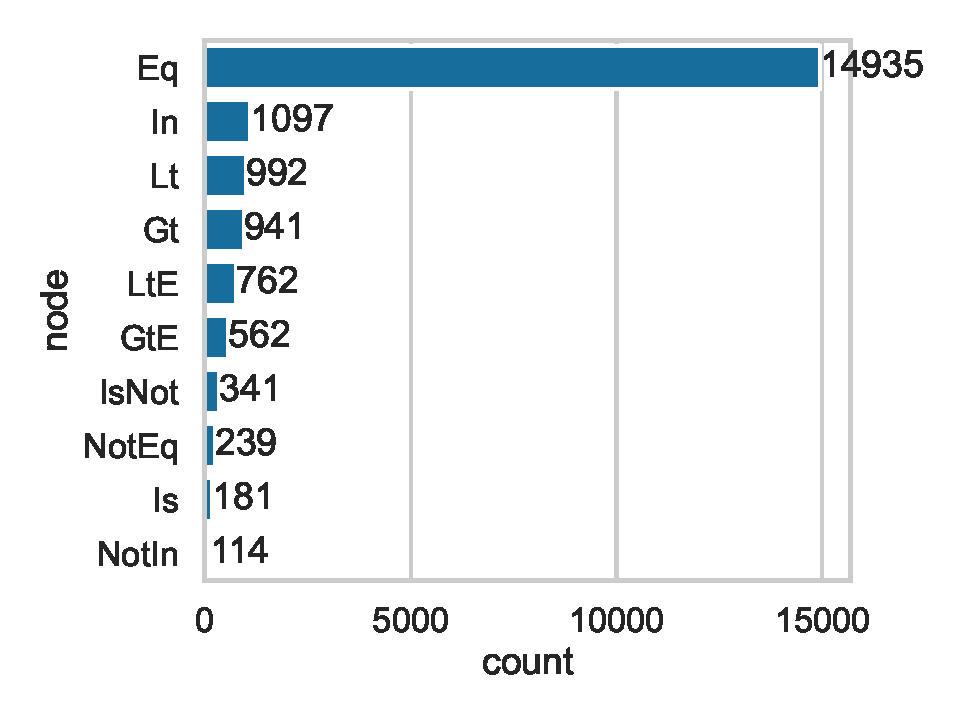
\includegraphics[width=\linewidth]{common-compare-op.pdf}
    \caption{10 most common operators used in \lstinline{assert} statements that perform a comparison check.}
    \label{fig:common-compare-op}
  \end{minipage}
\end{figure}

\begin{table}
  \centering
  \caption{Examples of the most common tests performed in assert statements.}
  \begin{tabular}{@{}m{0.5\textwidth} m{0.5\textwidth}@{}}
    \toprule
    \emph{\textbf{Comparison Check}}&
    \emph{\textbf{Function Call}}\\
    \midrule

    \lstinline[]$type(train_dataset[0]) == tuple$&
    \lstinline[]$(np.unique(y_test) == [-1, 1]).all()$\\

    \lstinline[]$torch.__version__ > '1.10.0'$&
    \lstinline[]$isinstance(transmat, pd.dataframe)$\\

    \lstinline[]$len(x_dev) == len(y_dev)$&
    \lstinline[]$np.allclose(np.linalg.norm(wio, axis=0), 1)$\\
    \bottomrule
  \end{tabular}
  \label{tab:common-assert-test}
\end{table}

We focus the remainder of the analysis on the 95\% of the assertions written using the \lstinline{assert} statement. The most common test performed in the \lstinline{assert} statements include a comparison check and a function call as shown in Figure~\ref{fig:common-assert-test}. Table~\ref{tab:common-assert-test} provides a few examples of assertions for each of the tests above. In Figure~\ref{fig:common-compare-op} we see the most common operators used in assert statements that perform a comparison check. We observe that overwhelming majority of the asserts ensure that two values are equal to each other. The shape and size of data structures are frequently compared as observed in Figure~\ref{fig:common-compare-lhs} and Figure~\ref{fig:common-compare-rhs} which show the most common bi-grams that appear in the LHS and RHS of the comparison statements respectively.

\begin{figure}
  \centering
  \begin{minipage}{0.49\textwidth}
    \centering
    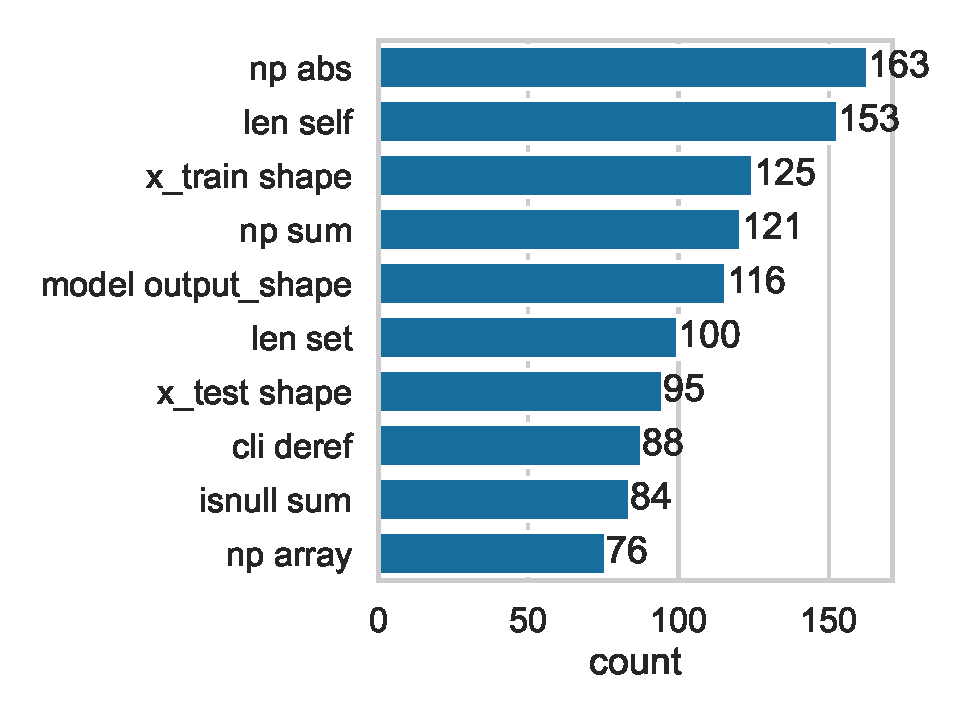
\includegraphics[width=\linewidth]{common-compare-lhs.pdf}
    \caption{Most common bi-grams that appear in the LHS of comparison statements.}
    \label{fig:common-compare-lhs}
  \end{minipage}
  \hfill
  \begin{minipage}{0.49\textwidth}
    \centering
    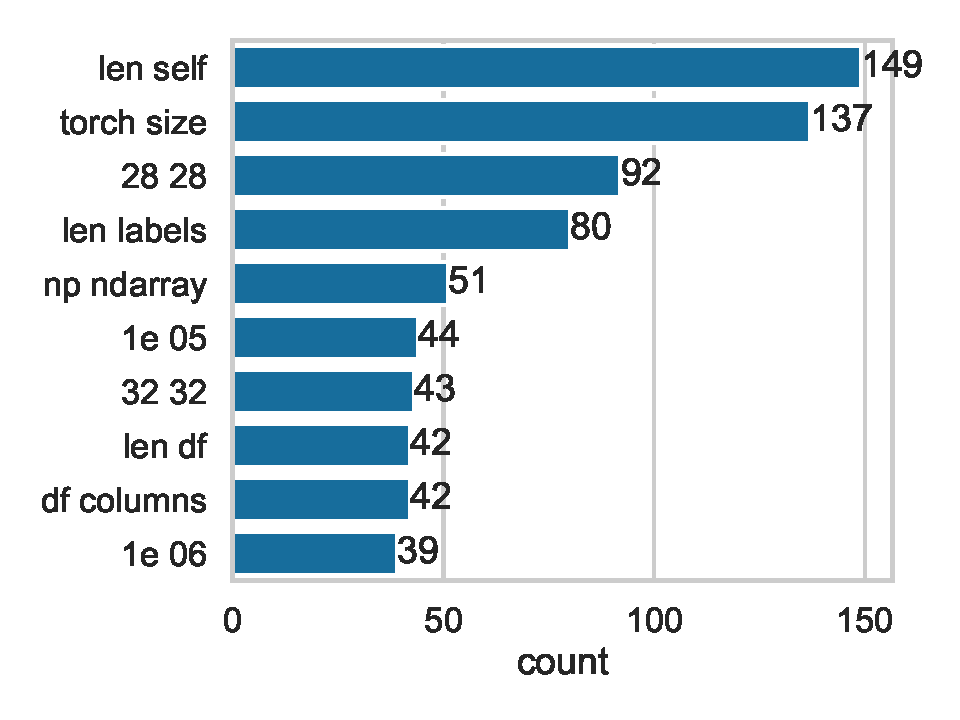
\includegraphics[width=\linewidth]{common-compare-rhs.pdf}
    \caption{Most common bi-grams that appear in the RHS of comparison statements.}
    \label{fig:common-compare-rhs}
  \end{minipage}
\end{figure}

Of the 95\% assert statements, 28.4 thousand (31.7\%) have a failure message. Figure~\ref{fig:common-assert-msgs} shows the most frequent bi-grams that appear in these failure messages. Similar to the analysis presented above, we removed the duplicate messages prior to analysing the bi-grams resulting in 5.9 thousand unique messages. The bi-grams indicate that the shape and data type of data structures are frequently verified.

\begin{figure}
  \centering
  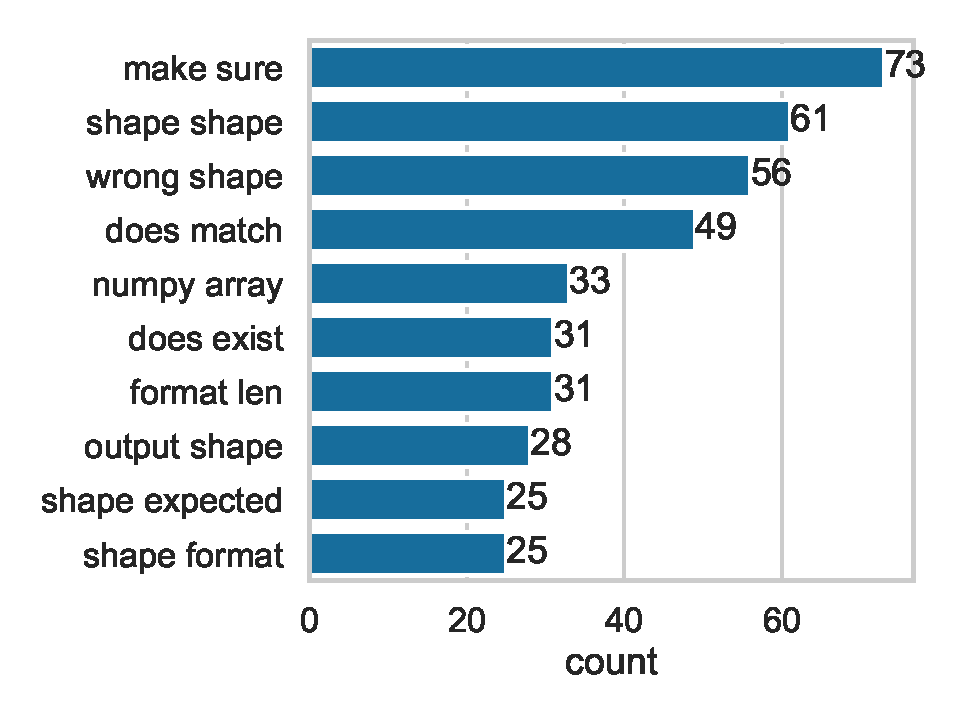
\includegraphics[width=0.5\textwidth]{common-assert-msgs.pdf}
  \caption{Most common bi-grams in the failure messages of assert statements.}
  \label{fig:common-assert-msgs}
\end{figure}

\begin{figure}
  \centering
  \begin{minipage}{0.49\textwidth}
    \centering
    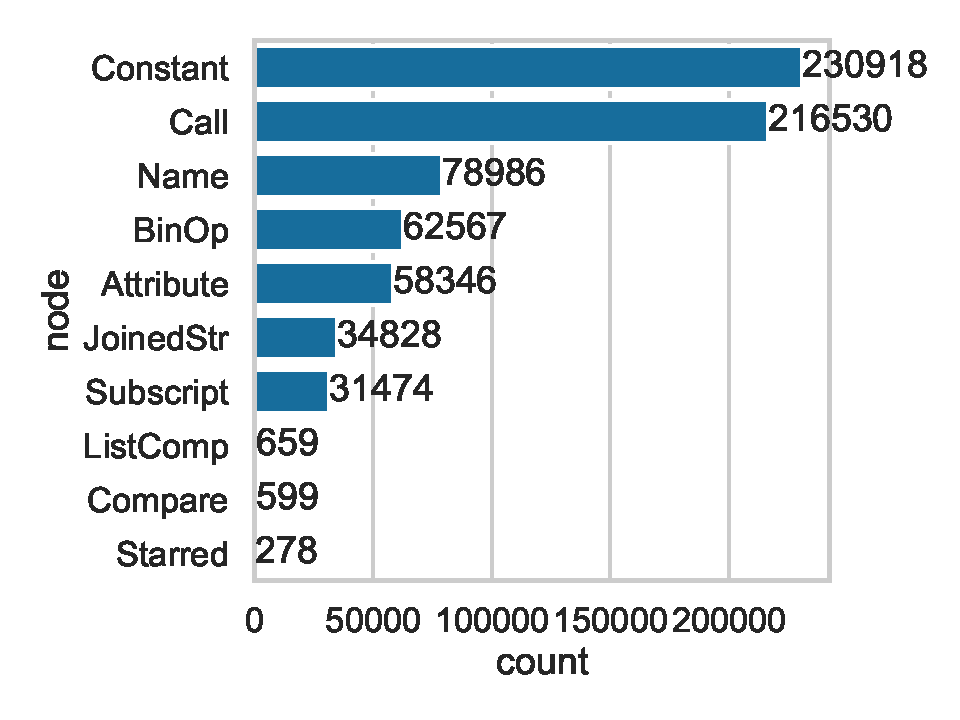
\includegraphics[width=\textwidth]{common-print-nodes.pdf}
    \caption{Most common AST nodes inside print statements}
    \label{fig:common-print-nodes}
  \end{minipage}
  \hfill
  \begin{minipage}{0.49\textwidth}
    \centering
    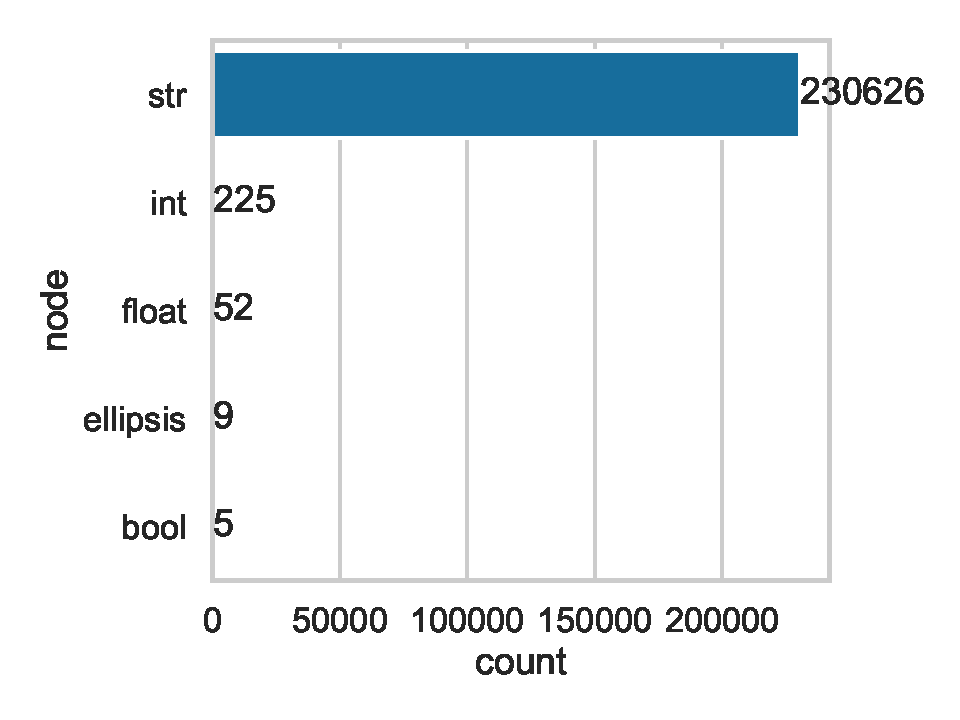
\includegraphics[width=\textwidth]{common-print-constant-types.pdf}
    \caption{Most common type of constant inside print statements}
    \label{fig:common-print-constant-types}
  \end{minipage}
\end{figure}

We collected 1.4 million print statements from 180 thousand notebooks (60\% of the total notebooks analysed in this study). Unlike assert statements, print statements do not have a fixed lexical semantic since the Python \lstinline{ast} module interprets them as regular function calls. Additionally, print statements can be written in several forms---the \lstinline{print} function may have multiple arguments, any form of string interpolation supported by Python or output from function calls. Figure~\ref{fig:common-print-nodes} shows that the most common AST nodes inside of print statements are constants followed by function calls. Figure~\ref{fig:common-print-constant-types} further validates that the constants are almost entirely of type string. Based on these observations, we disect the print statements into two components---text written in natural language (from the \emph{Constant} nodes) and code (from all other nodes). Figure~\ref{fig:common-print-constants} and Figure~\ref{fig:common-print-not-constants} present the most common bi-grams that appear in the natural text and code of print statements respectively. Both figures collectively indicate that print statements are frequently used to print various performance metrics of ML models.

\begin{figure}
  \centering
  \begin{minipage}{0.49\textwidth}
    \centering
    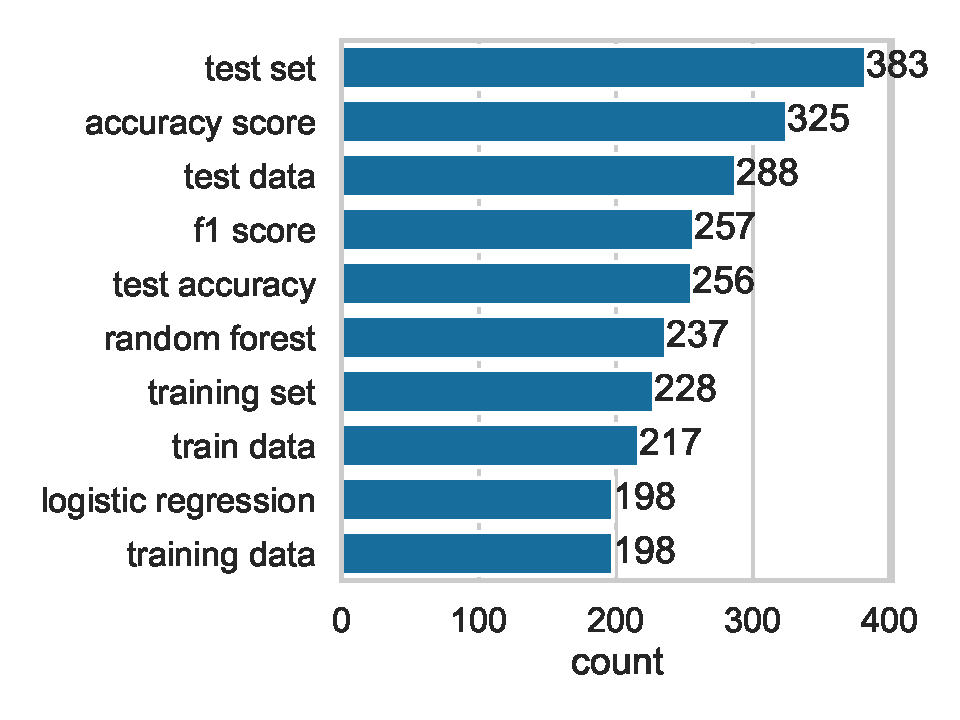
\includegraphics[width=\linewidth]{common-print-constants.pdf}
    \caption{Most common bi-grams that appear in natural text inside of print statements.}
    \label{fig:common-print-constants}
  \end{minipage}
  \hfill
  \begin{minipage}{0.49\textwidth}
    \centering
    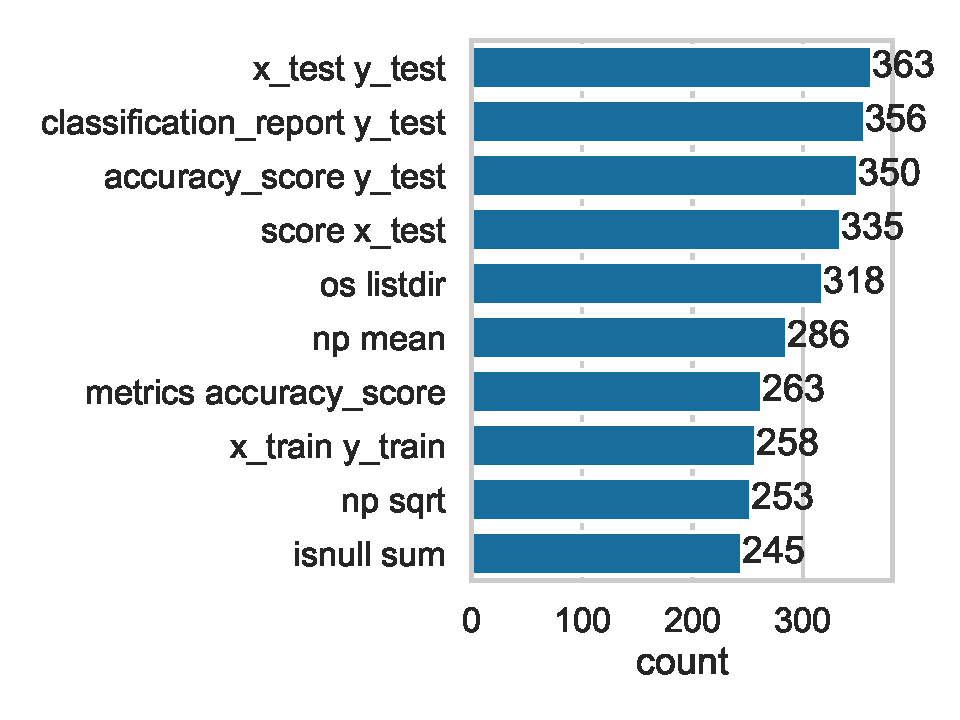
\includegraphics[width=\linewidth]{common-print-not-constants.pdf}
    \caption{Most common bi-grams that appear in the code of print statements.}
    \label{fig:common-print-not-constants}
  \end{minipage}
\end{figure}

We collected 1 million last statements from 119 thousand notebooks (40\% of the total notebooks analysed in this study). Figure~\ref{fig:common-last-nodes} shows that the most frequent type of code written as the final statement in a code cell is a function call. We further analyse the functions calls in more detail. Figure~\ref{fig:common-last-modules} and Figure~\ref{fig:common-last-functions} show the most modules and functions used inside the function calls respectively. The figures highlight the prominence of data visualisation libraries seaborn (\lstinline{sns}) and matplotlib (\lstinline{plt}) and visualisation functions such as \lstinline{plot} and \lstinline{countplot} in the notebooks. The data analysis tool pandas (represented by \lstinline{df} and \lstinline{pd}) also features prominently with many data exploration and preprocessing functions such as \lstinline{head}, \lstinline{value_counts} and \lstinline{describe} being used frequently. The presence of \lstinline{train} and \lstinline{model} modules along with the \lstinline{fit} function indicates the use of ML libraries.

\begin{figure}
  \centering
  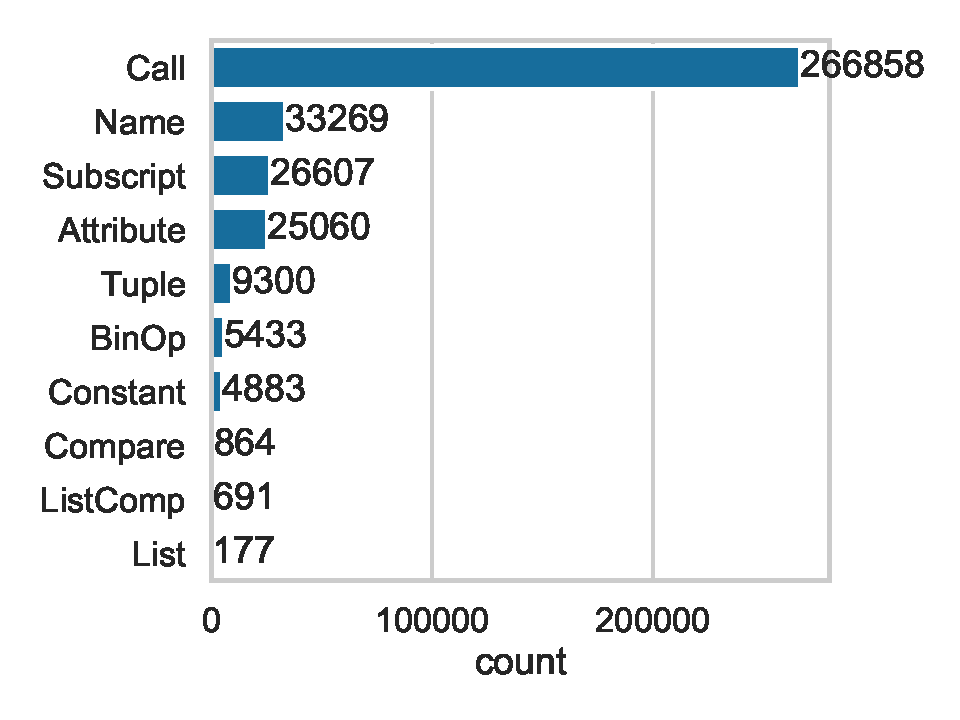
\includegraphics[width=0.5\textwidth]{common-last-nodes.pdf}
  \caption{Most common nodes in the last statement of code cells.}
  \label{fig:common-last-nodes}
\end{figure}

% TODO: we need better terminology here
\begin{figure}
  \centering
  \begin{minipage}{0.49\textwidth}
    \centering
    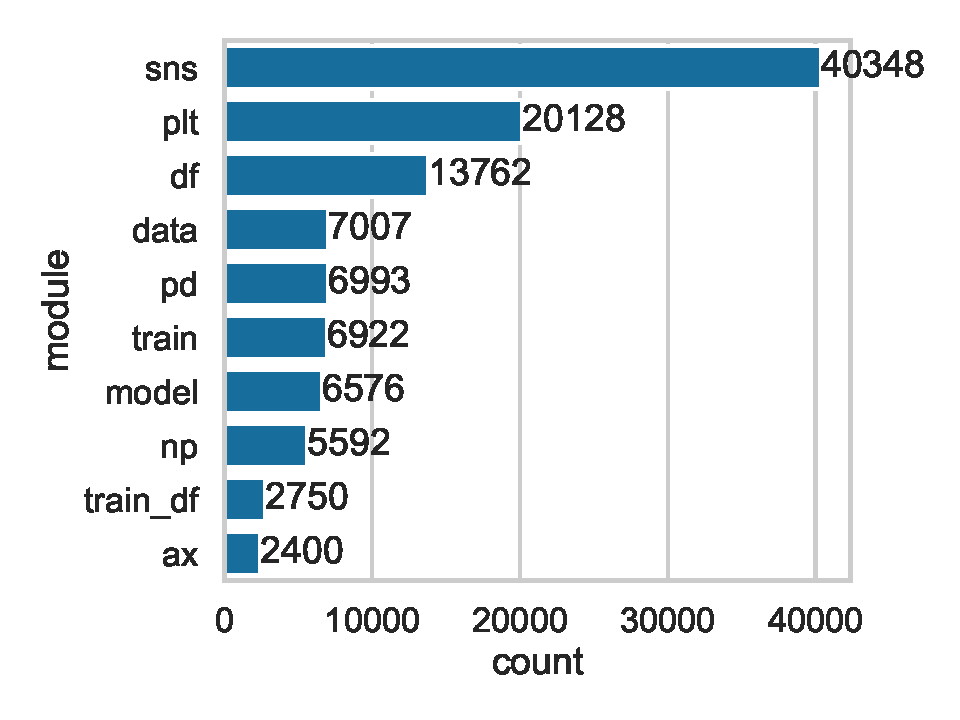
\includegraphics[width=\linewidth]{common-last-modules.pdf}
    \caption{Most common modules used in the function calls of last statements.}
    \label{fig:common-last-modules}
  \end{minipage}
  \hfill
  \begin{minipage}{0.49\textwidth}
    \centering
    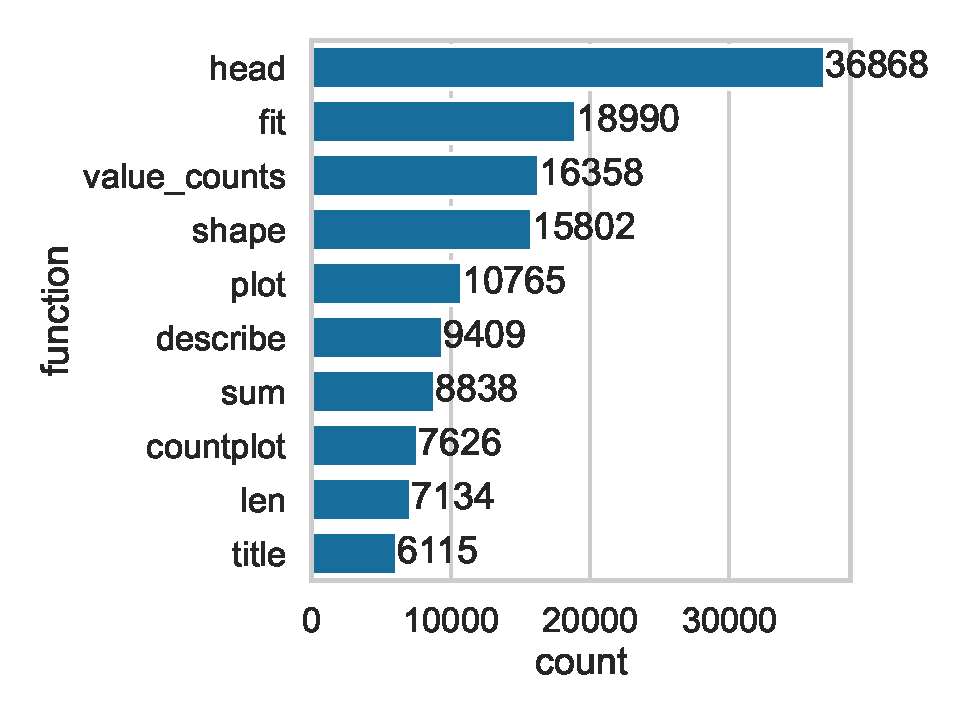
\includegraphics[width=\linewidth]{common-last-functions.pdf}
    \caption{Most common functions used in the function calls of last statements.}
    \label{fig:common-last-functions}
  \end{minipage}
\end{figure}

\begin{figure}
  \centering
  \begin{minipage}{0.49\textwidth}
    \centering
    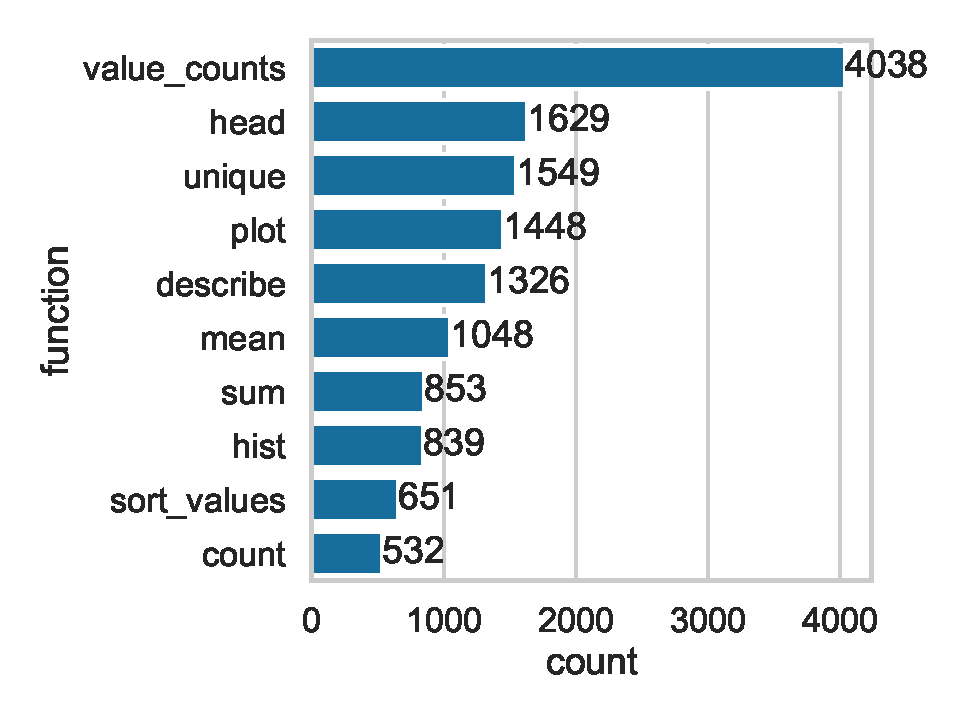
\includegraphics[width=\linewidth]{common-last-df-functions.pdf}
    \caption{Most common functions called on pandas data frames.}
    \label{fig:common-last-df-functions}
  \end{minipage}
  \hfill
  \begin{minipage}{0.49\textwidth}
    \centering
    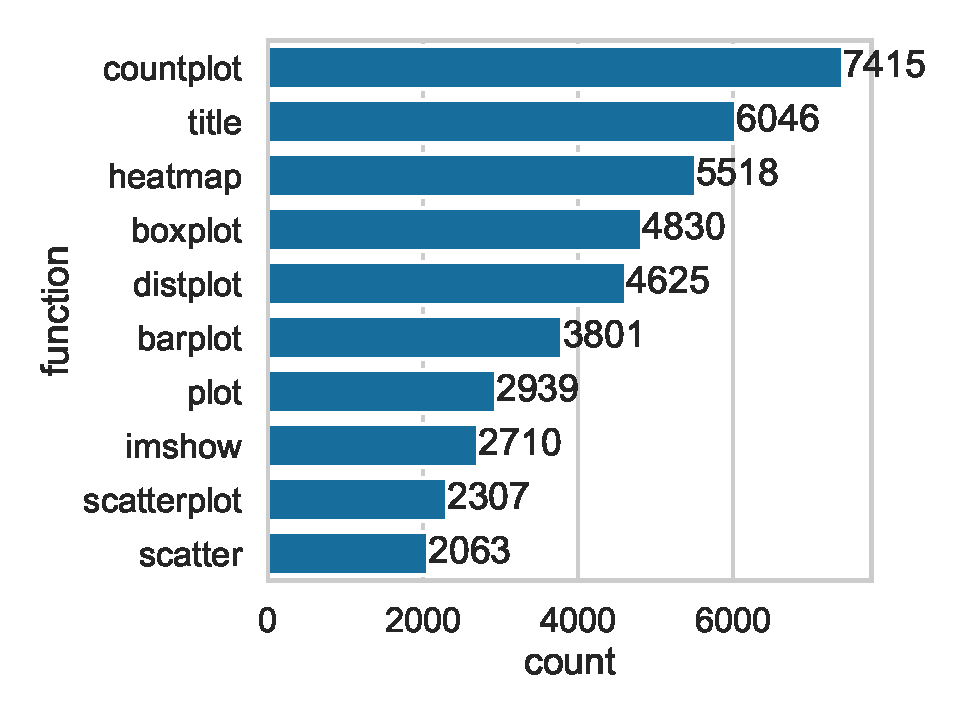
\includegraphics[width=\linewidth]{common-last-visualisation-functions.pdf}
    \caption{Most common visualisation functions used in last statements.}
    \label{fig:common-last-visualisation-functions}
  \end{minipage}
\end{figure}

We further analysed the most common functions called on pandas data frames by isolating the last statements where the module is \lstinline{data} or \lstinline{df}. This is shown in Figure~\ref{fig:common-last-df-functions} which reveals a focus on exploratory data analysis and statistical operations. The frequent use of functions such as \lstinline{value_counts}, \lstinline{head}, and \lstinline{unique}, indicate an emphasis on understanding the structure and content of the data. Visualisation functions like \lstinline{plot} and \lstinline{hist} suggest that practitioners often create quick visualisations directly from data frames. Descriptive statistics are also prominent, with functions like \lstinline{describe}, \lstinline{mean}, and \lstinline{sum} being commonly used.

Similarly, we also analysed the most common visualisation functions used in notebooks by isolating the last statements where the module is \lstinline{sns} or \lstinline{plt}. This is shown in Figure~\ref{fig:common-last-visualisation-functions} which indicates that categorical data visualisation appears to be a primary focus, with \lstinline{countplot} and \lstinline{barplot} ranking high among the most frequently used functions. The prominence of \lstinline{heatmap} and \lstinline{boxplot} functions indicates a regular need for visualising correlations and statistical distributions. For continuous data, functions like \lstinline{distplot}, \lstinline{scatterplot}, and \lstinline{scatter} are commonly used. The presence of \lstinline{imshow} suggests that image-related visualisations are also significant in many notebooks.

\subsection{(RQ2) How is explicit feedback from assert statements used to validate ML code written in Jupyter notebooks?}~\label{sec:result-explicit}

\subsubsection{Data shape check ($N = 26$)}
% (A5, A9, A13, A16, A17, A29, A31, A61, A71, A76--78, A82, A84, A85, A89, A90, A91, A93--96, A98--101)

Data shape checks can be considered the ``Swiss army knife'' of assertions, as they are ubiquitous and serve multiple purposes throughout the MLDL. We encountered a vast array of assert statements that verify the dimensions of various data structures, including input features (\emph{A17, A90}), labels (\emph{A5, A29}), predictions, images (\emph{A76, A93}), sequences, and embeddings (\emph{A76, A93}). These assertions ensure that the data adheres to the expected format and dimensions required by different components of the machine learning pipeline.

Data shape check assertions serve as a crucial safeguard against data inconsistencies, ensuring the integrity and compatibility of the data throughout the machine learning workflow. By verifying the expected dimensions and shapes of various data structures, these assertions help prevent runtime errors, ensure accurate model training and evaluation, and maintain the reliability of the entire machine learning pipeline.

\highlight{\textbf{Finding 2.1} 26 assertions verify the dimensions of various data structures such as input features, labels, predictions, images, sequences, and text embeddings. These checks ensure data consistency and compatibility throughout the ML pipeline, preventing runtime errors and ensuring accurate model training and evaluation.}

\subsubsection{Data validation check ($N = 14$)}
% formerly value-check (A20, A30, A41, A44--46, A52, A65, A68, A69, A73, A83, A87, A92)

We found assert statements that perform various validation checks on data structures, such as NumPy arrays and Pandas dataframes. These checks help ensure the data meets specific criteria or constraints, preventing potential errors or inconsistencies in downstream operations.

Common data validation checks include verifying the presence of specific values or ranges within arrays or columns(\emph{A41, A65}) and verifying the equality or closeness of arrays to a target value within a specified absolute tolerance (\emph{A44, A46}). Some assertions also focus on validating the uniqueness or cardinality of values (\emph{A52}) while others validate the presence of specific values or conditions within data structures (\emph{A73}).

By verifying specific conditions, value ranges, uniqueness, and equality constraints, these assertions help catch potential errors or inconsistencies early in the pipeline, preventing downstream issues and ensuring reliable and accurate results.

\highlight{\textbf{Finding 2.2} Fourteen assertions perform validation checks on data structures, ensuring the presence of specific values, verifying value ranges, and confirming uniqueness or cardinality of values. These checks catch potential errors or inconsistencies early, ensuring data meets specific criteria or constraints for robust ML applications.}

\subsubsection{Model performance check ($N = 11$)}\label{sec:assert-model-perf}
% (A7, A15, A19, A22, A24, A26, A38, A54, A58, A59, A72)

\begin{lstlisting}[caption={Assertion \emph{A58} used to check that the accuracy of a model is close to the specified value. The use of \lstinline{np.isclose} allows for small deviations in the accuracy thus accounting for the stocastic nature of ML models.}, label={lst:A58}]
assert np.isclose(accuracy, 0.9666666666666667)
\end{lstlisting}

This study finds several assertions used to test model performance against predefined thresholds for key metrics such as accuracy, precision, recall, F1 score, and others. Range checks confirm that the performance metrics fall within acceptable boundaries, indicating good predictive performance without overfitting (\emph{A38}). Direct comparisons of model outputs with expected results, validate the model's predictive accuracy and reliability under operational conditions (\emph{A15}). Other assertions ensure that the learned parameters align closely with theoretically or empirically derived values, further cementing the model’s statistical validity (\emph{A19}). Finally assertions are also used to check for the expected number of neighbours as an indirect measure of model performance in specifc scenarios like clustering (\emph{A7}).

The use of \lstinline{np.isclose} in Listing~\ref{lst:A58} is particularly noteworthy. This method accounts for the stochastic nature of many ML models, where slight variations in performance metrics can occur due to differences in initial conditions, random seed settings, or inherent randomness in algorithms. By allowing a small tolerance in the comparison, \lstinline{np.isclose} ensures that the model's performance is consistently close to the expected benchmark, thereby affirming its reliability despite the stochastic elements.

\highlight{\textbf{Finding 2.3} Eleven assertions evaluate model performance against predefined thresholds for accuracy, precision, recall, F1 score, and other metrics. These checks validate the model's predictive accuracy and reliability, ensuring it meets expected performance standards despite the stochastic nature of ML models.}

\subsubsection{Existence check ($N = 8$)}
% NOTE: this is a combination of missing-value-check and existence-check
% (A23, A42, A43, A50, A51, A63, A79, A86)

Existence checks are primarily used during the data preprocessing stage in the MLDL to ensure data integrity before analysis and modelling. These checks primarily focus on verifying the presence of necessary columns and the absence of missing values within those columns (\emph{A23, A42, A79, A86}). Such validations are especially crucial after data preprocessing steps, where transformations might inadvertently introduce \lstinline{NaN} values (\emph{A50, A51, A63}) or result in an empty dataframe (\emph{A43}). These checks are also crucial for maintaining the accuracy and efficiency of data handling processes, ensuring that the datasets are ready for robust ML applications.

\highlight{\textbf{Finding 2.4} Eight assertions ensure the presence of specific columns in the dataset and the absence of missing values. These checks prevent operations on empty datasets and confirm the absence of \texttt{NaN} values, maintaining data integrity and reliability for model training.}

\subsubsection{Resource check ($N = 7$)}~\label{sec:result-rq2-resource-check}
% (A10, A14, A18, A37, A60, A67 A74)

\begin{lstlisting}[caption={Assertion \emph{A37} used to ensure that an ML model has not reached an inconsistent state due to out-of-order or re-execution of code cells.}, label={lst:A37}]
assert svm.fit_status_ == 0, 'Forgot to train the SVM!'
\end{lstlisting}

Resource check assertions are used to ensure the availability and validity of essential resources, preventing runtime errors, and maintaining the integrity of the data, models, and visualisations. One set of assertions verify the existence of files on the file system, such as pre-trained models (\emph{A10}) or data files (\emph{A74}). Subsequently, assertions are employed to validate the successful loading of models (\emph{A14}) and the completion of model training processes (\emph{A37}).

A unique aspect of working with notebooks is the ability to re-run cells while experimenting, which can lead to unintended consequences. Aassertion \emph{A37} presented in Listing~\ref{lst:A37} addresses this scenario by checking if the SVM model has been properly trained before proceeding with further operations. This check prevents inconsistent model states from executing cells out of order or multiple times. Other interesting assertions unique to computational notebooks include verifying the presence of data in visualisations (\emph{A60}) and explicitly verifying the versions of critical libraries (\emph{A18, A67}).

\highlight{\textbf{Finding 2.5} Seven assertions confirm the availability of essential resources like pre-trained models, data files, successful model loading, and completion of training processes. These checks prevent runtime errors and ensure proper code execution, maintaining the reliability and robustness of the ML workflows.}

\subsubsection{Type check ($N = 5$)}
% (A2, A35, A40, A81, A88)

Type check assertions are used to maintain data integrity, ensure compatibility between different components of the ML pipeline, and preventing errors and unexpected behaviour. Type checks are commonly performed to ensure that the input features are PyTorch float tensors or NumPy arrays, a requirement for many deep learning models and scientific computing operations respectively (\emph{A2, A88}). Type checks are also applied to very the type of the ML models (\emph{A40}), data structures and intermediate objects (\emph{A35}) and individual columns or elements within a dataset (\emph{A81}).

\highlight{\textbf{Finding 2.6} Five assertions validate the data types of input features, models, and intermediate objects. These checks ensure compatibility with ML models and operations, preventing errors from incompatible methods or attributes, thus maintaining the reliability of the ML workflow.}

\subsubsection{Mathematical property check ($N = 4$)}
% (A3, A25, A56, A64)

When working with neural networks and other statistical models, it is imperative to ensure that mathematical properties are preserved throughout operations involving arrays and matrices. This rigour is captured though assertions that ensure convolution operations are dimensionally consistent (\emph{A3}), checking for the symmetry of matrices (\emph{A64}) and monitoring the standard deviation of outputs to decide the appropriateness of using batch normalisation (\emph{A25}). These assertions are not just precautionary but are vital for confirming that the underpinnings of ML algorithms align with expected mathematical principles.

\highlight{\textbf{Finding 2.7} Four assertions validate key mathematical properties of data and model outputs. These include ensuring dimensional consistency in convolution operations, monitoring standard deviation for batch normalization suitability, verifying uniformity in computations, and checking matrix symmetry. These checks confirm the robustness and reliability of model computations.}

\subsubsection{Batch size check ($N = 3$)}
% (A21, A28, A70)

In the context of neural networks, the practice of using batch processing is a key strategy to enhance computational efficiency and hardware utilisation. Batching stabilises the learning curve by updating the model weights based on the average gradient of a batch thereby optimising learning and enhancing generalisability of the model. Ensuring the batch size matches the hardware capacity is crucial to avoid memory overflow issues that can halt training. Assertions are used to check that the batch size divides evenly into the training dataset size which ensures that each training epoch is computationally efficient (\emph{A21}). Additionally, assertions are used to ensure that the size of the training data is larger than the batch size (\emph{A70}) and that image dimensions are suitably divisible by the patch size which is essential for certain convolutional networks (\emph{A28}).

\highlight{\textbf{Finding 2.8} This study identifies three assertions validating batch size configurations. These assertions ensure batch sizes are divisible by dataset sizes, image dimensions are appropriately divided by patch sizes, and the number of images exceeds the batch size. These checks are crucial for optimizing computational efficiency and ensuring stable and smooth model training.}

\subsubsection{Network architecture check ($N = 3$)}
% (A11, A62, A75)

When integrating pre-trained models or leveraging transfer learning techniques, it is crucial to ensure the compatibility of the custom neural network architecture with the pre-trained components. This is particularly important when combining convolutional layers from different sources, as the spatial dimensions and channel configurations must align correctly. Checks include the use of assertions to verify that the output and input dimensions of consecutive convolutional layers match (\emph{A11}), checking that shape of the activations have the right number of channels (\emph{A62}) and that the appropriate regularisation parameter is set (\emph{A75}). Such architectural checks are crucial for preventing potential issues during the forward pass of the neural network and ensuring that the custom and pre-trained components are compatible with each other.

\highlight{\textbf{Finding 2.9} Three assertions verify the consistency of neural network architecture. These include ensuring weight dimensions match across layers and that activation shapes and regularization parameters are as expected. These checks ensure that the neural network is correctly configured and integrated with pre-trained models, maintaining the integrity of data flow during training.}

\subsubsection{Data leakage check ($N = 1$)}
% (A33)

\begin{lstlisting}[caption={Assertion \emph{A33} used to ensure that the training and validation sets do not contain any overlapping values.}, label={lst:A33}]
assert len(
  set(tr_df.PetID.unique()).intersection(valid_df.PetID.unique())
) == 0
\end{lstlisting}

Ensuring the absence of data leakage between training and validation datasets is a fundamental best practice in ML to prevent overfitting. To guarantee that the model can generalise effectively to new examples, it is crucial to verify that the training and validation sets are completely distinct with no shared examples. By strictly separating these datasets, the validation phase provides an unbiased evaluation of the model's ability to generalise to data similar to, but not identical to that which it was trained on. This is demonstrated by Assertion \emph{A33} in Listing~\ref{lst:A33} ensures that there are no overlapping \lstinline{PetID} values between the training set and the validation set, thereby preventing any possibility of data leakage.

\highlight{\textbf{Finding 2.10} This study identifies one assertion to ensure there are no overlapping values between training and validation sets to prevent data leakage. Preventing data leakage is essential to avoid overfitting and ensure the model's ability to generalise to new data. This practice maintains the integrity and validity of the model evaluation metrics.}

\subsection{(RQ3) How is implicit feedback from print statements and last statements of code cells used when writing ML code in Jupyter notebooks?}~\label{sec:result-implicit}
% TODO: feedback from Luis
% -  up to this point I miss how exactly we plan to answer this question. Reading the results I get that we are answering by clustering outputs together based on their respective ML/DS task and then by analysing how that task is accomplished. We need to explain this either in the beginning of section 4.1 or in section 3

\subsubsection{Model performance check ($N = 33$)}
% (O3, O50, O52, O57, O74, P3, P6, P8--12, P16--19, P23, P24, P28, P30, P34, P42, P47, P48, P50, P51, P54, P55, P57, P58, P61, P78, P93)
% TODO: feedback from Luis
% - if needed, we can merge Excution time check here. (both execution time and model correctness can be presented as a KPI)

During the model development phase, the performance of an ML model is often printed to facilitate comparisons against other models or variations. Throughout this continuous experimentation phase, authors may adjust model parameters or modify the data by engineering new features. The model is then re-trained to check if these changes lead to performance improvements. Besides the \emph{accuracy} of the model (\emph{P3, P18}), we also see checks for the \emph{Root Mean Square Error (RMSE)} (\emph{P6}) and the use of the classification report (\emph{P50}) provided by scikit-learn~\footnote{https://scikit-learn.org/stable/modules/generated/sklearn.metrics.classification\_report.html} which reports the \emph{accuracy}, \emph{precision}, \emph{recall} and \emph{f1 score} for all labels present in the target feature. In addition, we find the use of heatmaps (\emph{L3}) to visualise the confusion matrix of a multi-label classification task and custom functions (\emph{L52}) to manually evaluate an image classification model on a random sample of input images.

\highlight{\textbf{Finding 3.1} The study identifies 33 outputs used to check the performance of trained ML models. These include outputs that print key performance metrics, a normalised heatmap used to visualise the confusion matrix of a model's predictions and a custom function written for manual evaluation of model predictions on random input samples. These checks are used throughout the iterative model development phase, enabling practitioners to compare different models or variations, adjust parameters, and refine features to improve performance.}

\subsubsection{Data distribution check ($N = 7$)}~\label{sec:data-distribution-output}
% (O2, O4, O9, O14, O20, O25, O48)

Understanding the distribution of data is crucial for making informed decisions about necessary transformation steps in data analysis. For instance, visualisations can efficiently determine if scaling, normalizing, or handling outliers is needed. During the exploratory data analysis phase, visualisations and pandas dataframes are commonly used to assess the distribution of specific columns (\emph{L9}), helping identify features related to the target variable (\emph{L2, L14})and informing feature inclusion in model training. Additionally, descriptive statistics are used post-transformation to manually verify the effectiveness of data transformation steps and ensuring that the data conforms to the expected format for further analysis (\emph{L48, L25}).

\highlight{\textbf{Finding 3.2} The study identifies seven outputs used to check data distribution, including visualisations like categorical plots, kernel density estimate plots and count plots, and statistical summaries from pandas dataframes. These checks are used for making informed decisions about data transformations such as scaling, normalising and handling outliers, ensuring data integrity and improving model training reliability during the exploratory data analysis phase.}

\subsubsection{Resource check ($N = 7$)}\label{sec:implicit-resource-check}
% (P71, P86, O64, O66, P68, P82, P107)

Similar to the assertions identified in Section~\ref{sec:result-rq2-resource-check}, we also find print and last cell statements that validate the availability of essential resources on the system where the notebooks are being executed. This includes checks for the availability of compute resources such as a GPU or a TPU (\emph{P68, P82, P86}), verifying that a dataset or a pre-trained model has been successfully loaded into memory (\emph{P107, L66}) and ensuring that a certain version of an external library is present on the system (\emph{P71}).

\highlight{\textbf{Finding 3.3} The study identifies seven outputs used to verify resource availability on the systems where the Jupyter notebooks are being executed. These checks include confirming the availability of compute resources like GPUs and TPUs, ensuring datasets or pre-trained models are successfully loaded, and verifying the presence of specific library versions. These checks are used for ensuring that the computational environment is correctly set up, preventing execution errors, and facilitating smooth workflow execution.}

\subsubsection{Spot check ($N = 5$)}
% (O56, O60, P64, P67, P114)

Performing value or spot checks can be an essential practice for ensuring data integrity and model accuracy at various stages of development. These checks are crucial for verifying that operations such as data transformations, model predictions, and feature engineering are functioning as expected. Common checks include verifying the number of features in the data matches expectations after applying feature selection or dimensionality reduction techniques (\emph{L60}), assessing the correctness of one-hot encoding (\emph{P114}) and ensuring that data retains its expected properties after manipulation (\emph{P64}).

\highlight{\textbf{Finding 3.4} This study finds five outputs used to perform spot checks at various stages of the MLDL. Spot checks are used to ensure data integrity by verifying data transformation and feature engineering steps meet expectations.}

\subsubsection{Model training check ($N = 4$)}
% (O8, O31, O42, P77)

During training it is common practice to monitor the progress periodically and use this feedback to adjustment training parameters or stop training early to prevent overfitting. This can be done by checking the best parameters found through tuning methods (\emph{L42}), fitting the model to the training data (\emph{L31}) or printing the training loss and accuracy to give real-time feedback on the learning efficacy of the model (\emph{L8}).

\highlight{\textbf{Finding 3.5} The study identifies four outputs used to monitor model training progress. These outputs provide real-time feedback on training loss and accuracy, validate model adherence to expected data patterns, and identify optimal parameters through tuning methods. These checks facilitate timely adjustments during the training process to prevent overfitting and ensure model performance optimization.}

\subsubsection{Missing value check ($N = 3$)}
% (O12, O36, P74)

Checking for missing values is a critical step in the preprocessing phase of an ML project because it significantly influences the quality and performance of the model. Missing data can lead to biased or incorrect conclusions if not handled properly, potentially skewing the model's performance by training on incomplete or non-representative samples~\cite{shome2022data}. Many ML algorithms demand complete numerical datasets to perform calculations such as matrix multiplication. Missing values interrupt these calculations, leading to errors or the inability to execute algorithms entirely. These checks can be performed in code (\emph{P74, L36}) and using visualisations such as a heatmap (\emph{L12}).

\highlight{\textbf{Finding 3.6} The study identifies three outputs used to check for missing data. Missing values can lead to biased or incorrect conclusions as many ML algorithms require complete numerical datasets for accurate calculations. Identifying and addressing missing data during preprocessing is essential to avoid errors and improve model reliability.}

\subsubsection{Shape check ($N = 3$)}
% (P4, P32, P117)

Ensuring that data dimensions align with expectations is important particularly following data pre-processing or transformation steps. Primarily, the number of features in the training set must match those in the testing set (\emph{P4, P32, P117}). This alignment is crucial because statistical ML models are trained on specific data dimensions and expect the same dimensional structure during inference to perform accurately. Similarly, in neural network architectures, the configuration of input layers depends directly on the shape of the training data, dictating the number of input neurons needed. Furthermore, the correspondence between the number of test examples and their respective labels is essential for accurately computing performance metrics.

\highlight{\textbf{Finding 3.7} The study identifies three outputs used to check the shape of data. These checks are used to ensure data dimensions align with expectations, particularly after preprocessing or transformation steps.}

\subsubsection{Data relationship check ($N = 2$)}~\label{sec:linear-relation-output}
% (O6, O10)

\begin{table}
  \centering
  \caption{Cell outputs used to verify linear relationship between features in the data.}
  \begin{tabular}{@{}m{0.05\textwidth} m{0.4\textwidth} m{0.4\textwidth}@{}}
    \toprule
    \emph{\textbf{Key}}&
    \emph{\textbf{Code}}&
    \emph{\textbf{Output}}\\
    \midrule

    L6&
    \lstinline[]$b = sns.relplot(x='SIZE', y='Cash', hue='CLARITY', alpha=0.9, palette='muted', height=8, data=raw_data)$&
    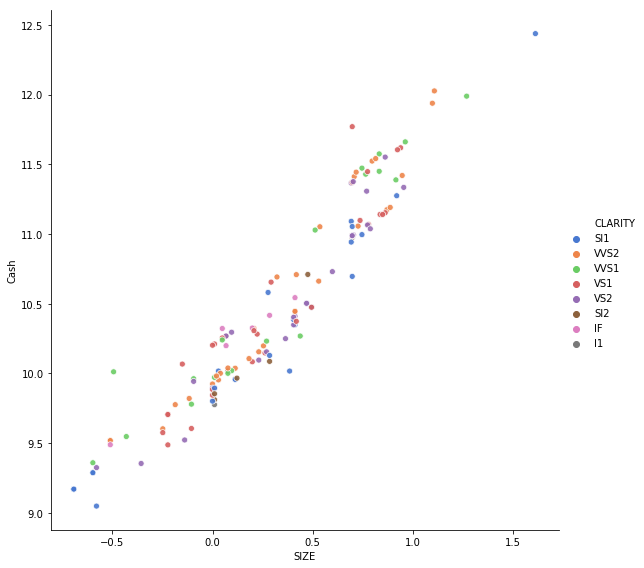
\includegraphics[width=\linewidth]{linear-relation-check-lineplot.png}\\

    L10&
    \lstinline[]$sns.regplot(x='X4 number of convenience stores', y='Y house price of unit area', data=data)$&
    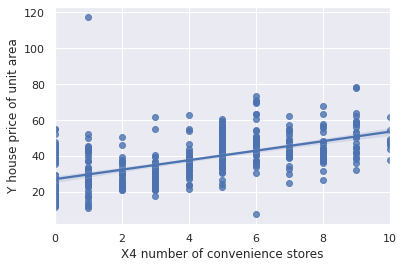
\includegraphics[width=\linewidth]{linear-relation-check-regplot.png}\\
    \bottomrule
  \end{tabular}
\label{tab:linear-relation-check}
\end{table}

Linear ML models achieve optimal performance when the target variable can be expressed as a linear combination of the input features. However, features within a dataset that exhibit a linear relationship are considered redundant as they convey the same information to the model during training. Consequently, the feature engineering stage often involves removing such features to create a more efficient training dataset~\cite{shome2022data}. Table~\ref{tab:linear-relation-check} illustrates two last cell statements found in this study for identifying linear relationships amongst features in the data. In addition to the code, the raw output of the cell is also shown since both case-studies produce a visualisation.  In \emph{L6}, the practitioner assesses the linearity between the features \texttt{Cash} and \texttt{SIZE}. \emph{L10} is a visualisation of the feature \texttt{X4} alongside the target variable \texttt{Y}, accompanied by a fitted linear regression model.

\highlight{\textbf{Finding 3.8} The study identifies two outputs used to verify linear relationships between features in the data. Visualisations such as a scatter plot with a regression line and a line plot are employed to assess the linearity between features. These checks are used for identifying and potentially removing redundant features or performing feature selection to ensure that the training dataset is optimized for linear ML models.}

\subsubsection{Type check ($N = 2$)}
% (O71, P43)

Type checks are crucial not only for confirming the current state of the data but also for determining the specific transformations required to make the data suitable for subsequent modelling steps. Ensuring data types align with model requirements is a fundamental step in the exploratory data analysis phase. Since all ML algorithms perform mathematical operations, they require the input data to be entirely numerical to avoid computational errors (\emph{P43, L71}). The process of checking data types helps in identifying the necessary pre-processing or transformation steps to convert the data into a form that is compatible with these models. For example, numerical features often require normalisation to bring them within a specific scale and categorical features must be converted into a numerical format through methods like one-hot encoding to ensure they can be effectively integrated into the model.

\highlight{\textbf{Finding 3.9} The study identifies two outputs used to verify the data types of features in the dataset. These checks are used to determine the necessary preprocessing or transformation steps requried to make the data suitable for training. Type checks are also used to ensure that all features are numerical prior to performing mathematical operations such as matrix multiplication, which is used in several ML models.}

\subsubsection{Execution time check ($N = 1$)}
% (P66)
\begin{lstlisting}[caption={Print statement \emph{P66} used to check the total execution time of training an ML model with various hyper-parameter configurations.}, label={lst:P66}]
print('Total Run Time:')
\end{lstlisting}

While training multiple ML models for a single task is common, choosing the best model considers not only its performance but also its training speed. Faster training times are more cost-effective for iterative tasks and promote sustainability in the long run~\cite{shome2022data}. Listing~\ref{lst:P66} presents print statement \emph{P66} that prints the total execution time of a code cell which trains an ML model with various hyper-parameter configurations using a grid-search. 

\highlight{\textbf{Finding 3.10} The study identifies one print statement used to check the total execution time of training and cross-validating an ML model. The print statement can be used to evaluate the efficiency of model training, especially when multiple models are trained iteratively.}

\subsubsection{Network architecture check ($N = 1$)}
% (P92)

Printing the structure of a neural network (\emph{P92}) serves crucial purposes such as verifying the correct implementation of the architecture, aiding in debugging by ensuring layer compatibility, and providing a clear, human-readable format for documentation and educational insights. It helps in verifying configurations like layer dimensions and operations before initiating computationally intensive training and ensuring that the model is set up efficiently for the intended tasks.

\highlight{\textbf{Finding 3.11} The study identifies one print statement used to show the architecture of a neural network. Such outputs can be used during the model development phase to ensure compatibility between the layers of a neural network, for understanding and learning about the architecture of pre-trained models and for documentation purposes.}

\section{Discussion}\label{sec:discuss}

Our results from RQ1 reveal that outputs from code cells in Jupyter notebooks are extensively used to make design and implementation decisions during the ML development cycle. Making such decisions however, requires manual validation of the outputs. For instance, we find several instances where practitioners use visualisations to check data distributions and print statements to verify data shapes and types before proceeding with model training. Critical decisions, such as deciding whether to normalize features based on their distributions or adjusting model parameters based on training feedback, rely heavily on these manual checks. Like traditional software systems, an ML pipeline is subject to change due to evolving model requirements, personnel turnover, and changes in the data itself. Such changes can introduce inconsistencies or errors that manual checks might miss, highlighting the need for more automated and explicit validation mechanisms.

Assertions can play a crucial role in automatically validating critical assumptions in ML workflows. As seen in the results from RQ2, assertions can verify that data distributions remain consistent with expectations or that model performance metrics meet predefined thresholds. Embedding assertions into the code helps ensure that any deviation from expected conditions is promptly flagged, reducing the reliance on manual verification and enhancing the robustness and maintainability of ML pipelines. Assertions also serve as an executable form of documentation that captures the assumptions and decisions made during model development. This is particularly important in collaborative environments where multiple practitioners might work on the same project. Assertions ensure that all team members have a clear understanding of the requirements and constraints across the entire ML pipeline, facilitating smoother transitions and handovers. Moreover, they enhance the reproducibility of ML experiments by ensuring that the same validation checks are applied consistently, regardless of the execution order of the notebook cells.

% P71 highlights the lack of proper software engineering best practices within Jupyter notebooks. This shortcoming in computational notebooks has been identified by prior studies~\cite{quaranta2021kgtorrent, pimentel2019large-scale}. In this case study, managing dependencies through external tools is recommended. Python's built-in \emph{requirements.txt}~\footnote{https://pip.pypa.io/en/stable/reference/requirements-file-format/} file allows specifying dependencies and versions. Alternatively, external programs like \emph{pipenv}~\footnote{https://pipenv.pypa.io/en/latest/} and \emph{poetry}~\footnote{https://python-poetry.org/} use lockfiles to ensure specific version control, guaranteeing reproducibility across different systems.

% NOTE: here we need to bring in prior literature on ML testing; and how majority of the research is working on testing using a test dataset; however we also have data and models
% NOTE: 3 pillars of of ML (sato2019continuous)

% TODO: feedback from Diomidis
% - "it represents an emerging testing practice within the ML community": I have commented before that assertions are different from tests. Assertions are a mechanism to increase the code's robustness, similar to type checks, array bounds checks, and thrown API exceptions.

From the 3 million Jupyter notebooks collected in this study, only 30 thousand (9.7\%) were found to utilize assertions. This indicates that while the use of assertions in Jupyter notebooks is still uncommon, it represents an emerging testing practice within the ML community. The relatively low adoption rate suggests that there is significant room for growth and improvement in the integration of assertions into ML development workflows.

We believe this limited use of assertions is due to a lack of knowledge among practitioners regarding testing approaches and the absence of adequate tooling to support the assertion of data and model properties. Current guidelines on ML coding practices require enhancement to emphasize the importance of testing. There is a pressing need to steer education and research in Software Engineering towards addressing the specific challenges faced when developing ML-enabled software systems. Fostering a deeper understanding of testing practices and providing tools tailored to ML development can help promote more rigorous and reliable testing methodologies within the community.

The assertions presented in RQ2 and RQ3 further reveal two significant challenges in the current landscape of testing in ML Jupyter notebooks. First, the assertions identified in this study lack the support of dedicated testing libraries. This suggests that the culture of testing ML code is still in its infancy, and ML practitioners are not yet fully exploring or leveraging software testing libraries. Secondly, existing testing libraries are not specifically tuned to the needs of ML code, leading practitioners to rely on basic built-in approaches. This highlights the necessity for developing specialized testing frameworks that cater to the unique requirements of ML projects.

Visualizations are an effective tool for interpreting complex ML models and data transformations. However, the manual effort required to validate insights derived from these visualizations can be substantially more compared to text output such as the ones presented in Section~\ref{sec:result-rq2}. We argue that the need for translating visual insights into formal assertions is more pressing. The visual cue and trends observed in visualisations are open to interpretation, thus the interpretation of the same plot may differ amongst two practitioners. Translating visual insights into assertions ensures that the knowledge encapsulated in the visualisations along with its interpretation and subsequent decisions made based on this interpretation is preserved and consistently applied throughout the ML lifecycle.

In the VA pairs from RQ3, we see several examples of assertions that fail to capture all the information gained from its visual counter-part. This can lead to a mismatch of expectations in future versions of the ML software. For instance, another project collaborator might run the code with a new version of the dataset or a different learning technique and assume that if the assertions run successfully, the expected patterns from the visualisation are also satisfied. The VA pairs presented in Section~\ref{sec:result-rq3} show that deriving assertions from visualisations is not trivial. Basic visualisation patterns require complex mathematical techniques which may be beyond the expertise of an ML developer. For example, a linear correlation between the true and predicted labels is evident in VA107 presented in Table~\ref{tab:va-model-perf}. Yet, its formal assertion necessitates defining an appropriate threshold for the coefficient of determination metric. Our results show that current software testing practices fail to capture the idiosyncrasies of ML code. There is a pressing need for automated tools, that bridge the disparity between the qualitative evaluation of ML systems using visualisations and the extraction of analytical assertions from these visuals.

% TODO: integrate our NLBSE paper
Our results show a clear need for developing ML-specific testing tools. Such tools should seamlessly integrate with computational notebooks and provide automated suggestions for assertions can greatly enhance the reliability and robustness of ML models. These tools can also aid in documenting and standardizing the use of domain-specific "magic" thresholds, ensuring that they are consistently applied and maintained.

% NOTE: we find overlap between the manual tests performed using the output of code cells and the assertions.

% NOTE: bring in prior work on reproducibility, code quality here
% NOTE: notebooks have been adopted by a much larger scientific community; not eveybody has a background in software engineering; we need more tools to aid notebook users...



\section{Implications}

% TODO: feedback from Diomidis
% - The implications section focuses implicitly on assertions, at the expense of the other elements discussed earlier.  Also, it puts excessive emphasis on testing, which IIUC is not the paper's topic.

\paragraph{\textbf{For ML developers}} ML developers are strongly encouraged to incorporate assertions into their Jupyter notebooks. Assertions play a crucial role in validating critical assumptions automatically, reducing the reliance on manual checks, and enhancing the robustness and maintainability of ML pipelines. By embedding assertions, developers can document the decisions made during model development, ensuring that these decisions are consistently applied and preserved throughout the ML lifecycle. This practice not only facilitates smoother transitions and handovers in collaborative environments but also improves the reproducibility of ML experiments by ensuring consistent validation checks.

\paragraph{\textbf{For Researchers}} The use of assertions in Jupyter notebooks, though currently uncommon, is an emerging testing practice within the ML community. This study highlights the potential for assertions to enhance the reliability and robustness of ML models by automating the validation of critical assumptions. Researchers are encouraged to explore the development and evaluation of ML-specific testing methodologies that leverage assertions. This could involve creating new testing frameworks and tools tailored to the unique challenges of ML systems, thus contributing to the advancement of software engineering practices in the ML domain.

\paragraph{\textbf{For Notebook Tool Developers}} There is a clear need for automated tools that suggest assertions based on the outputs of code cells in Jupyter notebooks. Tool developers can play a pivotal role by creating ML-specific testing tools that seamlessly integrate with computational notebooks. These tools should provide automated suggestions for assertions, helping practitioners to translate visual insights into formal, executable checks. By bridging the gap between qualitative evaluation and analytical assertions, such tools can significantly enhance the reliability and robustness of ML models, ensuring that they meet predefined performance standards consistently.

\paragraph{\textbf{For Educators}} Educators should emphasize the importance of testing ML code written in Jupyter notebooks as part of the curriculum. By incorporating testing practices and the use of assertions into ML education, students can develop a deeper understanding of the importance of automated validation in ensuring model reliability and robustness. Teaching these best practices early on can help cultivate a culture of rigorous testing among future ML practitioners, preparing them to address the specific challenges faced in ML-enabled software systems.

\paragraph{\textbf{For General Notebook Users}} Awareness of software engineering best practices, including the use of assertions, is crucial for all users of Jupyter notebooks. Assertions serve as an executable form of documentation, capturing the critical assumptions and decisions made during the development process. By adopting assertions, users can ensure that their notebooks are more robust, maintainable, and reproducible. This practice helps in maintaining consistency and reliability, especially in collaborative projects where multiple users might work on the same notebook, ensuring that the assumptions and validations are transparent and consistently applied.

\section{Threats to Validity}\label{sec:threats}

The empirical analysis presented in this study uses Jupyter notebooks mined from Github. To the best of our knowledge,~\emph{Pimentel et al} and~\emph{Quaranta et al} are the only two prior studies which provide a public dataset of Jupyter Notebooks. We faced several technical challenges while trying to access the notebooks provided by these replication packages and thus decided to mine our own data from Github. However, 24\% of the notebooks had to be excluded from the study since they were not related to ML or DS. We wish to extend our analysis to notebooks collected from Kaggle since it is predominantly targeted towards the ML and DS community.

In Section~\ref{sec:data-collect}, we intentionally keep the search criteria on Github broad by only checking for the appropriate file type and the presence of the ``assert'' keyword. Besides being used to define tests in the Python programming language, ``assert'' also appears in several external python testing libraries (for instance nose~\footnote{http://readthedocs.org/docs/nose/}, unittest~\footnote{https://docs.python.org/3/library/unittest.html} and numpy~\footnote{https://numpy.org/doc/stable/reference/routines.testing.html}). Our approach captures a rich variety of assertion statements while preventing the need to craft a custom search query based on an exhaustive list of keywords that appear in python testing libraries.

\section{Related Work}\label{sec:related}

% TODO: feedback from Diomidis
% - In Section 8 consider adding material regarind interactive ML development.

This section summarises prior scientific work that has been done in ML
Testing, computational notebooks and visual analytics. The section
concludes with an overview of technical knowledge required for this
paper.

\subsection{Assertions and Software Bugs}
 TODO

\subsection{Computational Notebooks and Software Engineering}\label{sec:notebooks}

\emph{Psallidas et al}~\cite{psallidas2019data} provide an overview of the evolving landscape of computational notebooks by analysing six million Python notebooks, two million enterprise Data Science (DS) pipelines, source code and metadata from over 900 releases of 12 important DS libraries. Their findings can be used by system builders for improving DS tools and also by DS practitioners to understand the current trends in technologies they should focus on. \emph{Pimentel et al}~\cite{pimentel2019large-scale} mined 1.4 million notebooks from Github to conduct an empirical study on the coding practices in computational notebooks. Based on their analysis, the authors propose guidelines on improving reproducibility of computational notebooks. To enable future research on computational notebooks, \emph{Quaranta et al}~\cite{quaranta2021kgtorrent} mine Kaggle and present \textit{KGTorrent}, a public dataset consisting of approximately 2.5 million Jupyter notebooks written in Python. The dataset also contains a relational database dump of metadata regarding publicly available notebooks on Kaggle.

Studies with human subjects have been conducted to gain a deeper understanding of the challenges faced by ML practitioners when developing ML models inside notebooks. The results indicate that ML practitioners work in a highly iterative fashion, often experimenting with multiple strategies to analyse the data or produce meaningful visualisations~\cite{kandel2012enterprise,kery2018story,liu2019understanding,chattopadhyay2020whats}. Studies have also been conducted to understand how practitioners generate, evaluate and manage alternative hypothesis, visual designs, methods, tools, algorithms and data sources to arrive at the final implementation~\cite{liu2019understanding,kandel2012enterprise}. The findings from these studies can be used as guidelines for improving existing notebook technologies or designing new ones.

To manage and prune multiple versions of code that accumulate over time when developing in notebooks, \emph{Head et al} propose a code gathering tool that allows practitioners to review and only keep the relevant version of code. Other tools such as \textit{WrangleDoc} and \textit{VizSmith} have also been proposed to aid ML practitioners when working within computational notebooks~\cite{yang2021subtle,bavishi2021vizsmith}.

Jupyter notebooks have been widely adopted by the DS and ML communities to develop ML pipelines~\cite{wang2020assessing,pimentel2019large-scale,quaranta2021kgtorrent}. Computational notebooks provide a rich source of data in the form of natural text, code and visualisations. Computational notebooks also allow ML practitioners to present the knowledge gained from the analysis in a narrative that can be shared with others~\cite{rule2018exploration}. This study leverages the computational narrative present within notebooks to identify visualisations and assertions that are semantically linked to each other.

\subsection{ML Testing}\label{sec:ml-testing}

% Testing ML enabled software systems poses more challenges compared to their traditional counter part. While traditional software systems mature through change in their codebase, ML enabled systems additionally experience change in the training data and the machine learning model~\cite{sculley2015hidden,amershi2019software,sambasivan2021everyone}. With ML being adopted into safety-critical domains that can affect human lives, ensuring that ML systems are correct, robust to data perturbations and not biased by race, colour or gender is of paramount importance.

Existing scientific literature on ML testing broadly focuses on two aspects. First, on functional properties such as correctness and robustness of the model towards unseen data. And second, on non-functional properties such as fairness, interpretability and privacy~\cite{zhang2020machine,mehrabi2021survey,chen2022fairness}.

To test the correctness of ML models, several improvements over existing test adequacy metrics have been proposed. Tools such as \textit{DeepXplore} and \textit{DeepGauge} propose new test adequacy metrics such as neuron coverage adapted for ML enabled software systems~\cite{pei2017deepxplore,ma2018deepgauge,gerasimou2020importance-driven}. Formal verification methods have also been proposed that try to provide formal guarantee of robustness against adversarial examples. Such methods however are only feasible for statistical ML models and become computationally expensive for more complex models such as deep neural networks~\cite{zhu2021deepmemory,baluta2021scalable}. Several works have been conducted on generating and detecting adversarial inputs for ML models. Data augmentation techniques based on fuzzing, search based software testing and mutation testing have been proposed to generate adversarial examples that can be used during model training to improve its robustness~\cite{braiek2019deepevolution,gao2020fuzz,wang2021robot,zhang2020white-box}. It is however not possible to include all variations of adversarial examples into the training data. Thus, methods have been proposed to detect adversarial inputs during runtime~\cite{xiao2021self-checking,wang2020dissector,wang2019adversarial,berend2020cats}.

In contrast to existing scientific contributions, we conduct a large-scale empirical analysis of Jupyter Notebooks to understand the process of testing ML systems. Specifically, we focus on how visualisations are used to test specific properties of ML systems. We further investigate how frequently analytical tests are formulated based on the information gained from the visualisations.

\subsection{Visualisations and Machine Learning}\label{sec:visualisations}

As ML augment software systems in safety-critical domains, emphasis has been put into explainability of ML models. ML models and the underlying data is complex and multi-dimensional. To combat the ``curse of dimensionality'', visual analytics has been widely adopted by the ML community to understand the data and the internal workings of ML models~\cite{yuan2021survey,hohman2019visual,wexler2019what-if}.

Prior studies have been conducted to understand how visual analytics techniques are currently being used in ML. \emph{Yuan et al} conduct a systematic review of 259 papers and propose a taxonomy of visual analytics techniques for ML. \emph{Hohman et al} conduct a survey of visual analytics techniques for Deep Learning Models. The findings of the study indicate that visual analytics has been widely adopted in ML for model explanation, interpretation, debugging and improvement.

Several tools have been proposed by the visual analytics research community to aid practitioners in understanding how their ML models operate. \emph{Wexler et al} propose \textit{What-If}, a visual analytics tool to explore alternative hypotheses, generate counterfactual reasoning, investigate decision boundaries of the model and how change in data affects the model predictions. To reduce the cognitive load of ML practitioners during model building phase, \emph{Amershi et al} propose \textit{ModelTracker}. Given a trained model and a sample dataset, ModelTracker presents all the information in traditional summary statistics along with the performance of the model.

\textit{ESCAPE}, \textit{GAM Coach}, \textit{Angler} and \textit{Drava} are a few other tools that have been proposed to handle specialised use-cases such as identifying systematic errors in ML models, generating counterfactual explanations for Generalised Additive Models, prioritising machine translation model improvements and relating human concepts with semantic dimensions extracted by ML models during disentangled representation learning\cite{ahn2023escape,wang2023gam,robertson2023angler,wang2023drava}.

In contrast to prior work which propose dedicated visual analytics tools, this study focuses on visualisations within computational notebooks. We focus on visualisations produced by AI practitioners using Python libraries (such as Matplotlib or Seaborn). Additional context provided by surrounding code and markdown cells are used to understand the motivation for creating the visualisation and the information gained from it.

\section{Conclusion and Future Work}

% NOTE: taxonomy of assertions mapping to V&V tasks in ML
% NOTE: automated tool that adds assertions once the contents of the NB is finalised?

This study empirically supports the efficacy of visualisations for testing various properties of machine learning systems. Visualisations enhance the ability of ML practitioners to interpret complex information through visual cues. However, decisions based on such visualisations demand manual verification in each development iteration. Analytical assertions derived from ML visualisations can reduce this manual effort by encapsulating key insights, and ensuring continuity in interpretation across different development stages and project collaborators.

Our results indicate that crafting analytical assertions from ML visualisations, is an emerging testing technique. Majority of the assertions however, are found to be primitive and unable to convey all information discerned from their visual counter-parts. This study finds a gap in the current software testing methods to address the unique challenges of ML. And emphasises the need for automated tools to bridge visual assessments and analytical assertions.

There is a clear need for tools designed to aid ML practitioners when testing ML systems. These tools should provide assistance in identifying the most suitable visualisations for testing specific properties of ML systems. Customized solutions that streamline the process of connecting visual insights to analytical assertions would significantly benefit practitioners in this domain.

The manual translation of insights derived from visualisations into analytical assertions presents a substantial challenge. Future work should focus on the development of automated tools that can assist AI practitioners in this translation process. Generating assertions from visual information automatically, will promote adoption of assertions in ML notebooks. And bring the code developed within notebooks, closer to a production-ready codebase.

% TODO remove this is no space left
Extending ML testing to dynamic real-world scenarios should be explored further. This entails developing techniques and frameworks that allow assertions to adapt to evolving data distributions, changing model requirements, and continuous system updates. Research in this area will contribute to the development of ML systems that remain reliable and relevant throughout their operational lifecycle.

% BibTeX users please use one of
% \bibliographystyle{spbasic}      % basic style, author-year citations
\bibliographystyle{spmpsci}      % mathematics and physical sciences
%\bibliographystyle{spphys}       % APS-like style for physics
\bibliography{bibliography}   % name your BibTeX data base

\end{document}
% end of file template.tex
